\chapter{Cross-loop Optimization of Arithmetic Intensity for Finite Element Local Assembly}
\label{ch:coffee}

\section{Introduction and Motivations}
In many fields such as computational fluid dynamics, computational electromagnetics and structural mechanics, phenomena are modelled by partial differential equations (PDEs). Numerical techniques, like the finite volume method and the finite element method, are widely employed to approximate solutions of these PDEs. Unstructured meshes are often used to discretize the computational domain, since they allow an accurate representation of complex geometries. The solution is sought by applying suitable numerical operations, or
kernels, to the entities of a mesh, such as edges, vertices, or cells. On standard clusters of multicores, typically, a kernel is executed sequentially by a thread, while parallelism is achieved by partitioning the mesh and assigning each partition to a different node or thread. Such an execution model, with minor variations, is adopted, for example, in \cite{pyop2isc}, \cite{Fenics}, \cite{fluidity_manual_v4}, \cite{lizst}.

The time required to apply the numerical kernels is a major issue, since the equation domain needs to be discretized into an extremely large number of cells to obtain a satisfactory approximation of the PDE, possibly of the order of trillions, as in \cite{Rossinelli2013}. For example, it has been well established that mesh resolution is critical in the accuracy of numerical weather forecasts. However, operational forecast centers have a strict time limit in which to produce a forecast - 60 minutes in the case of the UK Met Office. Producing efficient kernels has a direct scientific payoff in higher resolution, and therefore more accurate, forecasts. Computational cost is a dominant problem in computational science simulations, especially for those based on finite elements, which are the subject of this work. In this chapter, we address, in particular, the well-known problem of optimizing the local assembly phase of the finite element method, which can be responsible for a significant fraction of the overall computation run-time, often in the range 30-60$\%$ \citep{francis}, \citep{quadrature-olegaard}, \citep{petsc-integration-gpu}, \citep{tensor-kirby}. 

During the assembly phase, the solution of the PDE is approximated by executing a problem-specific kernel over all cells, or elements, in the discretized domain. We restrict our focus to relatively low order finite element methods, in which an assembly kernel's working set is usually small enough to fit the L1 cache. Low order methods are by no means exotic: they are employed in a wide variety of fields, including climate and ocean modeling, computational fluid dynamics, and structural mechanics. The efficient assembly of high order methods such as the spectral element method \citep{spencer} requires a significantly different loop nest structure. High order methods are therefore excluded from our study.

An assembly kernel is characterized by the presence of an affine, often non-perfect loop nest, in which individual loops are rather small: their trip count rarely exceeds 30, and may be as low as 3 for low order methods. In the innermost loop, a problem-specific, compute intensive expression evaluates a two dimensional array, representing the result of local assembly in an element of the discretized domain. With such a kernel structure, we focus on aspects like the minimization of floating-point operations, register allocation and instruction-level parallelism, especially in the form of SIMD vectorization.

We aim to maximize our impact on the platforms that are realistically used for finite element applications, so we target conventional CPU architectures rather than GPUs. 
The key limiting factor to the execution on GPUs is the stringent memory requirements. Only relatively small problems fit in a GPU memory, and support for distributed GPU execution in general purpose finite element frameworks is minimal. There has been some research on adapting local assembly to GPUs (mentioned later), although it differs from ours in several ways, including: (i) not relying on automated code generation from a domain-specific language (explained next), (ii) testing only very low order methods, (iii) not optimizing for cross-loop arithmetic intensity (the goal is rather effective multi-thread parallelization). In addition, our code transformations would drastically impact the GPU parallelization strategy, for example by increasing a thread's working set. For all these reasons, a study on extending the research to GPU architectures is beyond the scope of this work. In Section~\ref{sec:generality}, however, we provide some intuitions about this research direction.

Achieving high-performance on CPUs is non-trivial. The complexity of the mathematical expressions, often characterized by a large number of operations on constants and small matrices, makes it hard to determine a single or specific sequence of transformations that is successfully applicable to all problems. Loop trip counts are typically small and can vary significantly, which further exacerbates the issue. We will show that traditional vendor compilers, such as \emph{GNU's} and \emph{Intel's}, fail at exploiting the structure inherent such assembly expressions. Polyhedral-model-based source-to-source compilers, for instance~\cite{pluto}, can apply aggressive loop optimizations, such as tiling, but these are not particularly helpful in our context, as explained next. 

We focus on optimizing the performance of local assembly operations produced by automated code generation. This technique has been proved successful in the context of the FEniCS~\citep{Fenics} and Firedrake~\citep{firedrake-code} projects, become incredibly popular over the last years. In these frameworks, a mathematical model is expressed at high-level by means of a domain-specific language and a domain-specific compiler is used to produce a representation of local assembly operations (e.g. C code). \textit{Our aim is to obtain close-to-peak performance in all of the local assembly operations that such frameworks can produce}. Since the domain-specific language exposed to the users provide as constructs generic differential operators, an incredibly vast set of PDEs, possibly arising in completely different domains, can be expressed and solved. A compiler-based approach is, therefore, the only reasonable option to the problem of optimizing local assembly operations. 

Several studies have already tackled local assembly optimization in the context of automated code generation. In~\cite{quadrature-olegaard}, it is shown how this technique can be leveraged to introduce domain-specific optimizations, which a user cannot be expected to write ``by hand''. \cite{tensor-kirby} and~\cite{francis} have studied, instead, different optimization techniques based on a mathematical reformulation of the local assembly operations. The same problem has been addressed recently also for GPU architectures, for instance in~\cite{petsc-integration-gpu},~\cite{klockner-dg}, and~\cite{bana-ho-fem}. With our study, we make clear step forward by showing that different PDEs, on different platforms, require distinct sets of transformations if close-to-peak performance must be reached, and that low-level, domain-aware code transformations are essential to maximize instruction-level parallelism and register locality. As discussed in the following sections, our optimization strategy is quite different from those in previous work, although we reuse and leverage some of the ideas formulated in the available literature. 

We present a novel structured approach to the optimization of automatically-generated local assembly kernels. We argue that for complex, realistic PDEs, peak performance can be achieved only by passing through a two-step optimization procedure: 1) expression rewriting, to minimize floating point operations, 2) and code specialization, to ensure effective register utilization and instruction-level parallelism, especially SIMD vectorization. 

Expression rewriting consists of a framework capable of minimizing arithmetic intensity and optimize for register pressure. Our contribution is twofold:
\begin{itemize}
\item \emph{Rewrite rules for assembly expressions}. The goal is to the reduce the computational intensity of local assembly kernels by rescheduling arithmetic operations based on a set of rewrite rules. These aggressively exploit associativity, distributivity, and commutativity of operators to expose loop-invariant sub-expressions and SIMD vectorization opportunities to the code specialization stage. While rewriting an assembly expression, domain knowledge is used in several ways, for example to avoid redundant computation.
\item \emph{An algorithm to deschedule useless operations}. Relying on symbolic execution, this algorithm restructures the code so as to skip useless arithmetic operations, for example multiplication by scalar quantities which are statically known to be zero. One problem is to transform the code while preserving code vectorizability, which is solved by resorting to domain-knowledge. 
\end{itemize}

Code specialization's goal is to apply transformations to maximize the exploitation of the underlying platform's resources, e.g. SIMD lanes. We provide a number of contributions:
\begin{itemize}
\item \emph{Padding and data alignment}. The small size of the loop nest (integration, test, and trial functions loops) require all of the involved arrays to be padded to a multiple of the vector register length so as to maximize the effectiveness of SIMD code. Data alignment can be enforced as a consequence of padding. 
\item \emph{Vector-register Tiling}. Blocking at the level of vector registers, which we perform exploiting the specific memory access pattern of the assembly expressions (i.e. a domain-aware transformation), improves data locality beyond traditional unroll-and-jam optimizations. This is especially true for relatively high polynomial order (i.e. greater than 2) or when pre-multiplying functions are present.
\item \emph{Expression Splitting}. In certain assembly expressions the register pressure is significantly high: when the number of basis functions arrays (or, equivalently, temporaries introduced by loop-invariant code motion) and constants is large, spilling to L1 cache is a consequence for architectures with a relatively low number of logical registers (e.g. 16/32). We exploit sum's associativity to ``split'' the assembly expression into multiple sub-expressions, which are computed individually.
\item \emph{An algorithm to generate calls to BLAS routines}.
\item \emph{Autotuning}. We implement a model-driven, dynamic autotuner that transparently evaluates multiple sets of code transformations to determine the best optimization strategy for a given PDE. The main challenge here is to build, for a generic problem, a reasonably small search space that comprises most of the effective code variants.
\end{itemize} 

Expression rewriting and code specialization have been implemented in a compiler, COFFEE\footnote{COFFEE stands for COmpiler For Finit Element local assEmbly.}, fully integrated with the Firedrake framework~\cite{Luporini}. Besides separating the mathematical domain, captured by a domain-specific compiler at an higher level of abstraction, from the optimization process, COFFEE also aims to be platform-agnostic. The code transformations occur on an intermediate representation of the assembly operation, which is ultimately translated into platform-specific code. Domain knowledge is exploited in two ways: for simplifying the implementation of code transformations and to make them extremely effective. Domain knowledge is conveyed to COFFEE from the higher level through suitable annotations attached to the input. For example, when the input is in the form of an abstract syntax tree produced by the higher layer, specific nodes are decorated so as to drive the optimization process. Although COFFEE has been thought of as a multi-platform optimizing compiler, our performance evaluation so far has been restricted to standard CPU platforms only. We emphasize once more, however, that all of the transformations applicable would work on generic accelerators as well.

To demonstrate the effectiveness of our approach, we provide an extensive and unprecedented performance evaluation across a number of real-world PDEs of increasing complexity, including some based on complex hyperelasticity models. We characterize our problems by varying polynomial order of the employed function spaces and number of so called pre-multiplying functions. To clearly distinguish the improvements achieved by COFFEE, we will compare, for each examined PDE, four sets of code variants: 1) unoptimized code, i.e. a local assembly routine as returned from the domain-specific compiler; 2) code optimized by FEniCS, i.e. the work in~\cite{quadrature-olegaard}; 3) code optimized by expression rewriting and code specialization as described in this paper. Notable performance improvements of 3) over 1) and 2) are reported and discussed.

\section{Preliminaries}
\label{sec:coffee-preliminaries}
In this section, the basic concepts sustaining the finite element method are summarized. The notation adopted in~\cite{quadrature-olegaard} and~\cite{francis} is followed. At the end of this section, the reader is expected to understand what local assembly represents and how an implementation can be derived starting from a mathematical specification of the finite element problem. 

\subsection{Overview of the Finite Element Method}
We consider the weak formulation of a linear variational problem
\begin{equation}
\begin{split}
Find\ u\ \in U\ such\ that \\
a(u, v) = L(v), \forall v \in V
\end{split}
\end{equation}
where $a$ and $L$ are called bilinear and linear form, respectively. The set of \textit{trial} functions $U$ and the set of \textit{test} functions $V$ are discrete function spaces. For simplicity, we assume $U = V$ and $\lbrace \phi_i \rbrace$ be the set of basis functions spanning $U$. The unknown solution $u$ can be approximated as a linear combination of the basis functions $\lbrace \phi_i \rbrace$. From the solution of the following linear system it is possible to determine a set of coefficients to express $u$
\begin{equation}
A\textbf{u} = b
\end{equation}
in which $A$ and $b$ discretize $a$ and $L$ respectively:
\begin{equation}
\centering
\begin{split}
A_{ij} = a(\phi_i(x), \phi_j(x)) \\
b_i = L(\phi_i(x))
\end{split}
\end{equation}
The matrix $A$ and the vector $b$ are computed in the so called assembly phase. Then, in a subsequent phase, the linear system is solved, usually by means of an iterative method, and $\textbf{u}$ is eventually evaluated. 

We focus on the assembly phase, which is often characterized as a two-step procedure: \textit{local} and \textit{global} assembly. Optimizing the performance of local assembly is the subject of the research. Local assembly consists of computing the contributions that an element in the discretized domain provide to the approximated solution of the equation. Global assembly, on the other hand, is the process of suitably ``inserting'' such contributions in $A$ and $b$. 

\subsection{Quadrature Representation for Finite Element Local Assembly}
\label{sec:quadrature-rep}
Without loss of generality, we illustrate local assembly in a concrete example, the evaluation of the local element matrix for a Laplacian operator. Consider the weighted Laplace equation
\begin{equation}
- \nabla \cdot (w \nabla u) = 0
\end{equation}
in which $u$ is unknown, while $w$ is prescribed. The bilinear form associated with the weak variational form of the equation is:
\begin{equation}
a(v, u) = \int_\Omega w \nabla v \cdot \nabla u\ \mathrm{d}x
\end{equation}
The domain $\Omega$ of the equation is partitioned into a set of cells (elements) $T$ such that $\bigcup T = \Omega$ and $\bigcap T = \emptyset$. By defining $\lbrace \phi_i^K \rbrace$ as the set of local basis functions spanning $U$ on the element $K$, we can express the local element matrix as
\begin{equation}
\label{eq:stiffness}
A_{ij}^K = \int_K w \nabla \phi_i^K \cdot \nabla \phi_j^K\ \mathrm{d}x
\end{equation}
The local element vector $L$ can be determined in an analogous way starting from the linear form associated with the weak variational form of the equation. 

Quadrature schemes are conveniently used to numerically evaluate $A_{ij}^K$. For convenience, a reference element $K_0$ and an affine mapping $F_K : K_0 \rightarrow K$ to any element $K \in T$ are introduced. This implies a change of variables from reference coordinates $X_0$ to real coordinates $x = F_K (X_0)$ is necessary any time a new element is evaluated. The numerical integration routine based on quadrature representation over an element $K$ can be expressed as follows
\begin{equation}
\label{eq:quadrature}
\scriptsize
A_{ij}^K = \sum_{q=1}^N \sum_{\alpha_3=1}^n \phi_{\alpha_3}(X^q)w_{\alpha_3} \sum_{\alpha_1=1}^d \sum_{\alpha_2=1}^d \sum_{\beta=1}^d \frac{\partial X_{\alpha_1}}{\partial x_{\beta}} \frac{\partial \phi_i^K(X^q)}{\partial X_{\alpha_1}} \frac{\partial X_{\alpha_2}}{\partial x_{\beta}} \frac{\partial \phi_j^K(X^q)}{\partial X_{\alpha_2}} det F_K' W^q
\end{equation}
where $N$ is the number of integration points, $W^q$ the quadrature weight at the integration point $X^q$, $d$ is the dimension of $\Omega$, $n$ the number of degrees of freedom associated to the local basis functions, and $det$ the determinant of the Jacobian matrix used for the aforementioned change of coordinates.  

In the next sections, we will often refer to the local element matrix evaluation, such as Equation~\ref{eq:quadrature} for the weighted Lapalce operator, as the \textit{assembly expression} deriving from the weak variational problem.

\subsection{Implementation of Quadrature-based Local Assembly}
\subsubsection{From Math to Code}
We have explained that local assembly is the computation of contributions of a specific cell in the discretized domain to the linear system which yields the PDE solution. The process consists of numerically evaluating problem-specific integrals to produce a matrix and a vector (only the derivation of the matrix was shown in Section~\ref{sec:quadrature-rep}), whose sizes depend on the order of the method. This operation is applied to all cells in the discretized domain (mesh).

We consider again the weighted Laplace example of the previous section. A C-code implementation of Equation~\ref{eq:quadrature} is illustrated in Listing~\ref{code:weighted-laplace}. The values at the various quadrature points of basis functions ($\phi$) derivatives are tabulated in the FE0$\_$D10 and FE0$\_$D01 arrays. The summation along quadrature points $q$ is implemented by the \emph{i} loop, whereas the one along $\alpha_3$ is represented by the \emph{r} loop. In this example, we assume $d=2$ (2D mesh), so the summations along $\alpha_1$, $\alpha_2$ and $\beta$ have been straightforwardly expanded in the expression that evaluates the local element matrix $A$. 

\begin{algorithm}
\scriptsize
\SetAlgorithmName{LISTING}{}

\KwSty{void} weighted$\_$laplace(\KwSty{double} A[3][3], \KwSty{double} **coordinates, \KwSty{double} **w) \\
$\lbrace$ \\
~~  // Compute Jacobian \\
~~  \KwSty{double} J[4]; \\
~~  compute$\_$jacobian$\_$triangle$\_$2d(J, coordinates); \\
~~\\
~~  // Compute Jacobian inverse and determinant \\
~~  \KwSty{double} K[4]; \\
~~  \KwSty{double} detJ; \\
~~  compute$\_$jacobian$\_$inverse$\_$triangle$\_$2d(K, detJ, J); \\
~~  \KwSty{const double} det = fabs(detJ); \\
~~\\
~~  // Quadrature weights \\
~~  \KwSty{static const double} W1[1] = {0.5}; \\
~~\\
~~  // Basis functions \\
~~  \KwSty{static const double} FE0$\_$D10[1][3] = $\lbrace\lbrace$ -0.999999999999999, ...$\rbrace\rbrace$ ;\\
~~  \KwSty{static const double} FE0$\_$D01[1][3] = $\lbrace\lbrace$ -1.0, ...$\rbrace\rbrace$ ;\\
~~  \KwSty{static const double} FE0[1][3] = $\lbrace\lbrace$ 0.333333333333333, ...$\rbrace\rbrace$ ;\\
~~\\
~~  \KwSty{for} (\KwSty{int} i = 0; i < 6; ++i)\\
~~  $\lbrace$\\
~~~~  \KwSty{double} F0  = 0.0;\\
~~~~  \KwSty{for} (\KwSty{int} r  = 0; r < 3; ++r)\\
~~~~~~  F0 += (w[r][0] * FE0[i][r]);\\
~~\\
~~~~  \KwSty{for} (\KwSty{int} j = 0; j < 3; ++j)\\
~~~~~~    \KwSty{for} (\KwSty{int} k = 0; k < 3; ++k)\\
~~~~~~~~      A[j][k] += (\underline{(}\textbf{(}((K[1]*FE0$\_$D10[i][k])+(K[3]*FE0$\_$D01[i][k])) * \\
~~~~~~~~~~~~~~~~~~~~~~~~~~~~((K[1]*FE0$\_$D10[i][j])+(K[3]*FE0$\_$D01[i][j]))\textbf{)} + \\
~~~~~~~~~~~~~~~~~~~~~~~~~~~~\textbf{(}((K[0]*FE0$\_$D10[i][k])+(K[2]*FE0$\_$D01[i][k])) * \\
~~~~~~~~~~~~~~~~~~~~~~~~~~~~((K[0]*FE0$\_$D10[i][j])+(K[2]*FE0$\_$D01[i][j]))\textbf{)}\underline{)}*det*W1[i]*F0);\\
~~  $\rbrace$\\
$\rbrace$
\caption{A possible implementation of Equation~\ref{eq:quadrature} assuming a 2D triangular mesh and polynomial order $q=2$ Lagrange basis functions.}
\label{code:weighted-laplace}
\end{algorithm}

More complex assembly expressions, due to the employment of particular differential operators in the original PDE, are obviously possible. Intuitively, as the complexity of the PDE grows, the implementation of local assembly becomes increasingly more complicated. This fact is actually the real motivation behind reasearch in automated code generation techniques, such as those used by state-of-the-art frameworks like FEniCS and Firedrake. Automated code generation allows scientists to express the finite element specfication using a domain-specific language resembling mathematical notation, and obtain with no effort a semantically correct implementation of local assembly. The research in the present work is about making such an implementation also extremely effective, in terms of run-time performance, on standard CPU architectures. 

\begin{algorithm}
\scriptsize
\SetAlgorithmName{LISTING}{}

// This is a Firedrake construct (\textbf{not} an UFL's) to instantiate a 2D mesh.\\
mesh = UnitSquareMesh(size, size)\\
// FunctionSpace also belongs to the Firedrake language \\
V = FunctionSpace(mesh, "Lagrange", 2)\\
u = \KwSty{TrialFunction}(V)\\
v = \KwSty{TestFunction}(V)\\
weight = \KwSty{Function(V)}.\KwSty{assign}(value)\\
a = weight\KwSty{*}\KwSty{dot}(\KwSty{grad}(v), \KwSty{grad}(u))\KwSty{*dx}
\caption{UFL specification of the weighted Laplace equation for polynomial order $q=2$ Lagrange basis functions.}
\label{code:weighted-laplace-ufl}
\end{algorithm}

The domain-specific language used by Firedrake and FEniCS to express finite element problems is the Unified Form Language (UFL) \citep{ufl}. Listing~\ref{code:weighted-laplace-ufl} shows a possible UFL implementation for the weighted Laplace form. Note the resemblance of \emph{a = weight*...} with Equation~\ref{eq:stiffness}. A form compiler translates UFL code into the C code shown in Listing~\ref{code:weighted-laplace}. We will describe these aspects carefully in Section~\ref{sec:coffee-implementation}; for the moment, this level of detail sufficies to open a discussion on how to optimize local assembly kernels arising from generic partial differential equations.

\subsubsection{Other Examples and Motivations for Optimizations}
\label{sec:coffe-motivations}

\begin{figure}
\begin{alltt}
\scriptsize
\textbf{Input:} element matrix (2D array, initialized to 0), coordinates (array), 
       coefficients (array, e.g. velocity)
\textbf{Output:} element matrix (2D array)
- Compute Jacobian from coordinates
- Define basis functions
- Compute element matrix in an affine loop nest
\end{alltt}
\caption{Structure of a local assembly kernel}
\label{code:general-structure}
\end{figure}

%The code transformations described in this work are also
%generalizable to non-Firedrake assembly kernels, provided that the
%same numerical integration algorithm is employed.

The structure of a local assembly kernel can be generalized as in Figure~\ref{code:general-structure}. The inputs are a zero-initialized two dimensional array used to store the element matrix, the element's coordinates in the discretized domain, and coefficient fields, for instance indicating the values of velocity or pressure in the element. The output is the evaluated element matrix. The kernel body can be logically split into three parts:
\begin{enumerate}
  \item Calculation of the Jacobian matrix, its determinant and its
    inverse required for the aforementioned change of coordinates from
    the reference element to the one being computed.
  % FIXME: this rather hand-wavy and not technically correct
  \item Definition of basis functions used to interpolate fields at the
    quadrature points in the element. The choice of basis functions is
    expressed in UFL directly by users. In the generated code, they are
    represented as global read-only two dimensional arrays (i.e., using
    \texttt{static const} in C) of double precision floats.
  \item Evaluation of the element matrix in an affine loop nest, in which
    the integration is performed.
\end{enumerate}
Table~\ref{table:map-name-letters} shows the variable names we will use in the upcoming code snippets to refer to the various kernel objects.

\begin{table}
\scriptsize
\begin{center}
\begin{tabulary}{1.0\columnwidth}{C|C|C}
\hline
Object name & Type & Variable name(s) \\\hline
Determinant of the Jacobian matrix & double & det  \\
Inverse of the Jacobian matrix & double & K1, K2, ... \\
Coordinates & double** & coords\\
Fields (coefficients) & double** & w \\
Numerical integration weights & double[] & W \\
Basis functions (and derivatives) & double[][] & X, Y, X1, ... \\
Element matrix & double[][] & A\\ \hline
\end{tabulary}
\end{center}
\caption{Type and variable names used in the various listings to identify local assembly objects.}
\label{table:map-name-letters}
\end{table}

%JUNK SENTENCES: Since only the values assumed at the integration
%points are needed to compute the element matrix, a basis function is
%implemented as a two dimensional array of double precision
%floats. The same basis functions can be used to evaluate all element
%matrices, provided that a suitable change of coordinates from a
%``reference'' element to a real one is performed. Therefore, basis
%functions are declared in the kernel body as global read-only arrays
%(i.e., using \texttt{static const} in C), rather than passed as
%function parameters. Basis functions are chosen at the UFL layer
%based on the problem being solved, so they are actually an input to
%the code generator.

\begin{algorithm}[t]
\scriptsize
\SetAlgorithmName{LISTING}{}

\KwSty{void} helmholtz(\KwSty{double} A[3][3], \KwSty{double} **coords) $\lbrace$\\
~~// K, det = Compute Jacobian (coords) \\
~~\\
~~\KwSty{static const double} W[3] = $\lbrace$...$\rbrace$\\
~~\KwSty{static const double} X$\_$D10[3][3] = $\lbrace\lbrace$...$\rbrace\rbrace$\\
~~\KwSty{static const double} X$\_$D01[3][3] = $\lbrace\lbrace$...$\rbrace\rbrace$\\
~~\\
~~\KwSty{for} (\KwSty{int} i = 0; i$<$3; i++) \\
~~~~\KwSty{for} (\KwSty{int} j = 0; j$<$3; j++) \\
~~~~~~\KwSty{for} (\KwSty{int} k = 0; k$<$3; k++) \\
~~~~~~~~A[j][k] += ((Y[i][k]*Y[i][j]+\\
~~~~~~~~~~~+((K1*X$\_$D10[i][k]+K3*X$\_$D01[i][k])*(K1*X$\_$D10[i][j]+K3*X$\_$D01[i][j]))+\\
~~~~~~~~~~~+((K0*X$\_$D10[i][k]+K2*X$\_$D01[i][k])*(K0*X$\_$D10[i][j]+K2*X$\_$D01[i][j])))*\\
~~~~~~~~~~~*det*W[i]);\\
$\rbrace$
\caption{Local assembly implementation for a Helmholtz problem on a 2D mesh using polynomial order $q=1$ Lagrange basis functions.}
\label{code:helmholtz}
\end{algorithm}

\begin{algorithm}[t]
\scriptsize
\SetAlgorithmName{LISTING}{}

\KwSty{void} burgers(\KwSty{double} A[12][12], \KwSty{double} **coords, \KwSty{double} **w) $\lbrace$\\
~~// K, det = Compute Jacobian (coords) \\
~~\\
~~\KwSty{static const double} W[5] = $\lbrace$...$\rbrace$\\
~~\KwSty{static const double} X1$\_$D001[5][12] = $\lbrace\lbrace$...$\rbrace\rbrace$\\
~~\KwSty{static const double} X2$\_$D001[5][12] = $\lbrace\lbrace$...$\rbrace\rbrace$\\
~~//11 other basis functions definitions.\\
~~...\\
~~\KwSty{for} (\KwSty{int} i = 0; i$<$5; i++) $\lbrace$\\
~~~~\KwSty{double} F0 = 0.0;\\
~~~~//10 other declarations (F1, F2,...)\\
~~~~...\\
~~~~\KwSty{for} (\KwSty{int} r = 0; r$<$12; r++) $\lbrace$\\
~~~~~~F0 += (w[r][0]*X1$\_$D100[i][r]);\\
~~~~~~//10 analogous statements (F1, F2, ...)\\
~~~~~~...\\
~~~~$\rbrace$\\
~~~~\KwSty{for} (\KwSty{int} j = 0; j$<$12; j++) \\
~~~~~~\KwSty{for} (\KwSty{int} k = 0; k$<$12; k++) \\
~~~~~~~~A[j][k] += (..(K5*F9)+(K8*F10))*Y1[i][j])+\\
~~~~~~~~~+(((K0*X1$\_$D100[i][k])+(K3*X1$\_$D010[i][k])+(K6*X1$\_$D001[i][k]))*Y2[i][j]))*F11)+\\
~~~~~~~~~+(..((K2*X2$\_$D100[i][k])+...+(K8*X2$\_$D001[i][k]))*((K2*X2$\_$D100[i][j])+...+(K8*X2$\_$D001[i][j]))..)+\\
~~~~~~~~~+ $<$roughly a hundred sum/muls go here$>$)..)*\\
~~~~~~~~~*det*W[i]);\\
~~$\rbrace$ \\
$\rbrace$
\caption{Local assembly implementation for a Burgers problem on a 3D mesh using polynomial order $q=1$ Lagrange basis functions.}
\label{code:burgers}
\end{algorithm}

The actual complexity of a local assembly kernel depends on the finite element problem being solved. In simpler cases, the loop nest is perfect, has short trip counts (in the range 3--15), and the computation reduces to a summation of a few products involving basis functions. An example is provided in Listing~\ref{code:helmholtz}, which shows the assembly kernel for a Helmholtz problem using Lagrange basis functions on 2D elements with polynomial order $q=1$. In other scenarios, for instance when solving the Burgers equation, the number of arrays involved in the computation of the element matrix can be much larger. The assembly code is given in Listing~\ref{code:burgers} and contains 14 unique arrays that are accessed, where the same array can be referenced multiple times within the same expression. This may also require the evaluation of constants in outer loops (called $F$ in the code) to act as scaling factors of arrays. Trip counts grow proportionally to the order of the method and arrays may be block-sparse.

In general, the variations in the structure of mathematical expressions and in loop trip counts (although typically limited to the order of tens of iterations) that different equations show, render the optimization process challenging, requiring distinct sets of transformations to bring performance closest to the machine peak. For example, the Burgers problem, given the large number of arrays accessed, suffers from high register pressure, whereas the Helmholtz equation does not. Moreover, arrays in Burgers are block-sparse due to the use of vector-valued basis functions (we will elaborate on this in the next sections). These few aspects (we could actually find more) already intuitively suggests that the two problems require a different treatment, based on an in-depth analysis of both data and iteration spaces. Furthermore, domain knowledge enables transformations that a general-purpose compiler could not apply, making the optimization space even larger. In this context, our goal is to understand the relationship between distinct code transformations, their impact on cross-loop arithmetic intensity, and to what extent their composability is effective in a wide class of real-world equations and architectures.

We also note that despite the infinite variety of assembly kernels that frameworks like FEniCS and Firedrake can generate, it is still possible to identify common domain-specific traits that are potentially exploitable for our optimization strategy. These include: 1) memory accesses along the three loop dimensions are always unit stride; 2) the \texttt{j} and \texttt{k} loops are interchangeable, whereas interchanges involving the $i$ loop require pre-computation of values (e.g. the $F$ values in Burgers) and introduction of temporary arrays (explained next); 3) depending on the problem being solved, the \texttt{j} and \texttt{k} loops could iterate along the same iteration space; 4) most of the sub-expressions on the right hand side of the element matrix computation depend on just two loops (either \texttt{i}-\texttt{j} or \texttt{i}-\texttt{k}). In the following sections we show how to exploit these observations to define a set of systematic, composable optimizations.

%TODO: more observations are needed here: e.g. linear algebra operations...

\section{Overview of the Optimization Strategy}

To generate high performance implementation of local assembly kernels, assembly expressions must be optimized with regards to three interrelated aspects: 
\begin{itemize}
\item arithmetic intensity
\item instruction-level parallelism
\item data locality
\end{itemize}
Three conceptually distinct kind of transformations can be individuated, which we refer to as \textit{expression rewriting}, \textit{code specialization}, and \textit{general-purpose optimizations}. Expression rewriting mainly targets arithmetic intensity by transforming the assembly expression (and its enclosing loop nest) so as to minimize the number of floating point operations required to evaluate the local element matrix. Code specialization is tailored to optimizing for instruction-level parallelism, particularly SIMD vectorization, and data (register) locality. Both classes of transformations are inspired by the inherent structure of local assembly code and make use of domain knowledge: as elaborated in the next sections, these two aspects are the core motivations for which standard general-purpose compilers fail at maximizing the performance of local assembly kernels. The third class of transformations is about general-purpose optimizations; that is, generic, well-known techniques for improving code performance, such as loop unrolling or loop interchange, that for some reasons are not applied by the compiler generating machine code, but potentially useful in certain equations.

In Sections~\ref{sec:coffee-expr-rewrite}--\ref{sec:coffee-genpurp-opts}, these classes of code transformations are presented. In Section~\ref{sec:coffee-implementation}, it is explained that their application to local assembly kernels must follow a specific order to ensure the correctness of the resulting code. Some effort was invested in ensuring that optimizations at stage $i$ (e.g. expression rewriting) would not break any further optimization opportunity at stage $i+1$ (code specialization). The theory and the implementation of a technique to select the optimal combination of transformations for a given equation are finally discussed.

% Need to mention composability here

\section{Expression Rewriting}
\label{sec:coffee-expr-rewrite}

Expression rewriting is about exploiting properties of operators such as associativity, distributivity, and commutativity, to minimize arithmetic intensity, expose code vectorization opportunities, and optimize the register pressure in the various levels of the assembly loop nest. There are many possibilities of rewriting an expression, so the transformation space can be quite large. Firstly, in Sections~\ref{sec:coffee-licm}--\ref{sec:coffee-expansion}, several ways of manipulating an assembly expression and their potential impact on the computational cost are described. Then, in Section~\ref{sec:coffee-rewrite-rules}, a simple yet systematic way of rewriting an expression based on a set of formal rewrite rules, which is the key to effectively explore the expression's transformation space, is formalized. 

The second objective of expression rewriting (Section~\ref{sec:coffee-avoidzeros}) consists of re-structuring the iteration space so as to avoid arithmetic operations over zero-valued columns in block-sparse basis functions arrays. Zero-valued columns arise, for example, when taking derivatives on a reference element or when using mixed (vector-valued) elements. This problem was tackled in~\cite{quadrature-olegaard}, but the proposed solution, which makes use of indirection arrays in the generated local assembly code, breaks most of the optimizations applicable by code specialization, including the fundamental SIMD vectorization. The contribution of the present research is a novel domain-aware approach based on symbolic execution that avoids indirection arrays.

\subsection{Generalized Loop-invariant Code Motion}
\label{sec:coffee-licm}

\begin{figure}
\centering
\label{code:original-code}
\footnotesize
\lstinputlisting{coffee/listings/simple.code}
\caption{Original (simplified) code}
\end{figure}

Consider the local element matrix computation in Figure~\ref{code:original-code}, which is an excerpt from the Burgers problem shown in Listing~\ref{code:burgers}. The assembly expression, produced by the FEniCS and Firedrake's form compiler, has been deliberately simplified, and code details have been omitted for brevity and readability. In practice, as already emphasized, assembly expressions can be much more complex depending on the differential operators employed in the variational form; however, this example is representative enough for highlighting patterns that are common in a large class of equations. 

A first glimpse of the code suggests that the \texttt{a*f0*A[i][j]+b*f1*B[i][j]} sub-expression is invariant with respect to the innermost (trial functions) loop \texttt{k}, so it can be hoisted at the level of the outer loop \texttt{j} to avoid redundant computation. This is indeed a standard compiler transformation, supported by any available compilers, so, in principle, there should be no need to transform the source code explicitly. With a closer look we notice that the sub-expression \texttt{d*D[i][k]+e*E[i][k]} is also invariant, although, this time, with respect to the outer (test functions) loop \texttt{j}. Available compilers (e.g. \emph{GNU's} and \emph{Intel's}) limit the search for code motion opportunities to the innermost loop of a given nest. Moreover, the hoisted code is scalar and therefore not subjected to SIMD auto-vectorization. In other words, these general-purpose compilers lack performance models to determine (i) the optimal place where to hoist an expression and (ii) the potential gain and overhead (due to the need for extra temporary memory) of vectorization. These are notable limitations for local assembly kernels. 

\begin{figure}
\centering
\label{code:invariant-code}
\footnotesize
\lstinputlisting{coffee/listings/invariant.code}
\caption{Invariant code}
\end{figure}

We work around these limitations with source-level loop-invariant code motion. In particular, we pre-compute all values that an invariant sub-expression assumes along its fastest varying dimension. This is implemented by introducing a temporary array per invariant sub-expression and by adding a new loop to the nest. At the price of extra memory for storing temporaries, the gain is that lifted terms can be auto-vectorized as part of an inner loop. Given the short trip counts of our loops, it is important to achieve auto-vectorization of hoisted terms in order to minimize the percentage of scalar instructions, which could otherwise be significant. It is also worth noting that, in some problems, for instance Helmholtz in Listing~\ref{code:helmholtz}, invariant sub-expressions along \texttt{j} are identical to those along \texttt{k}, and both loops iterate over the same iteration space, as anticipated in Section~\ref{sec:coffe-motivations}. In these cases, we safely avoid redundant pre-computation. The resulting code for the running Burgers example is shown in Figure~\ref{code:invariant-code}.

In the following, we refer to this series of transformations as \textit{generalized loop-invariant code motion}. We will show that this optimization is crucial when optimizing non-trivial assembly expressions, allowing to achieve performance improvements over the original code larger than 3$\times$.


\subsection{Terms Factorization}
\label{sec:coffee-factorize}

\begin{figure}
\centering
\label{code:factorized-code}
\footnotesize
\lstinputlisting{coffee/listings/factorized.code}
\caption{Factorized code}
\end{figure}

After generalized loop-invariant code motion has been applied, some assembly expressions can still  ``hide'' opportunities for code hoisting. By examining again the code in Figure~\ref{code:invariant-code}, we notice that the basis function array \texttt{A} iterating along the \texttt{[i,j]} loops appears twice in the expression. By expanding the products in which \texttt{A} is accessed and by applying sum commutativity, terms can be factorized. This has two effects: firstly, it reduces the number of arithmetic operations performed; secondly, and most importantly, it exposes a new sub-expression \texttt{A[i][k]/c+T2[k]*f} invariant with respect to loop \texttt{j}. Consequently, hoisting can be performed, resulting in the code in Figure~\ref{code:factorized-code}. In general, exposing factorization opportunities requires traversing the whole expression tree, and then expanding and moving terms. It also needs heuristics to select a factorization strategy: there may be different opportunities of reorganizing sub-expressions, and, in our case, the best is the one that maximizes the invariant code eventually disclosed. We will discuss this aspect formally in Section~\ref{sec:coffee-rewrite-rules}.

\subsection{Precomputation of Invariant Terms}
\label{sec:coffee-precompute}

\begin{figure}
\centering
\label{code:scalarexp-code}
\footnotesize
\lstinputlisting{coffee/listings/vectexpanded.code}
\caption{Scalar-expanded code}
\end{figure}

We note that integration-dependent expressions are inherently executed as scalar code. For example, the \texttt{f0*a} and \texttt{f1*b} products in Figure~\ref{code:factorized-code} depend on the loop along quadrature points; these operations are performed in a non-vectorized way at every \texttt{i} iteration. This is not a big issue in our running example, in which the scalar computation represents a small fraction of the total, but it becomes a concrete problem in complicated forms, like those at the heart of hyperelasticity (which will be part of our performance evaluation). In such forms, the amount of computation independent of both test and trial functions loops is so large that it has a significant impact on the run-time, despite being executed only $O(I)$ times (with $I$ number of quadrature points). We have therefore implemented an algorithm to move and scalar-expand integration-dependent expressions, which leads to codes as in Figure~\ref{code:scalarexp-code}.

\subsection{Expanding Sub-expressions}
\label{sec:coffee-expansion}

Expression rewriting also aims at minimizing register pressure in the assembly loop nest. Once the code has been optimized for arithmetic intensity, it is important to think about how the transformations impacted register allocation. Assume the local assembly kernel is executed on a state-of-the-art CPU architecture having 16 logical registers, e.g. an Intel Haswell. Each value appearing in the expression is loaded and kept in a register as long as possible. In Figure~\ref{code:scalarexp-code}, for instance, the scalar value \texttt{g} is loaded once, whereas the term \texttt{det*W[i]} is precomputed and loaded in a register at every \texttt{i} iteration. This implies that at every iteration of the \texttt{[j,k]} loop nest, 12$\%$ of the available registers are spent just to store values independent of test and trial functions loops. In more complicated expressions, the percentage of registers destined to store such constant terms can be even higher. Registers are, however, a precious resource, especially when evaluating compute-intensive expressions. The smaller is the number of available free registers, the worse is the instruction-level parallelism achieved: for example, a shortage of registers can increase the pressure on the L1 cache (i.e. it can worsen data locality), or it may prevent the effective application of standard transformations, e.g. loop unrolling. We aim at relieving this problem by suitably expanding terms and introducing, where necessary, additional temporary values. We illustrate this in the following example.

%An analogous analysis applies to processors with larger numbers of registers, since using loop unroll or loop unroll-and-jam to expose more instruction-level parallelism would increase the requirements on registers.

\begin{figure}
\footnotesize
\subfigure[Original (simplified) code]{\label{code:toexpand-code}\lstinputlisting{coffee/listings/toexpand.code}}
~\\
~\\
\subfigure[The code after expansion of \texttt{det*W[i]}]{\label{code:expanded-1-code}\lstinputlisting{coffee/listings/expanded-1.code}}
~\\
~\\
\subfigure[The code after expansion of \texttt{g}. Note the need to introduce a new temporary array.]{\label{code:expanded-2-code}\lstinputlisting{coffee/listings/expanded-2.code}}
\caption{Expansion of terms to improve register pressure in a local assembly kernel}\label{code:expanded-code}
\end{figure}

Consider a variant of the Burgers local assembly kernel, shown in Figure~\ref{code:toexpand-code}. This is again a representative, simplified example. We can easily distribute \texttt{det*W[i]} over the three operands on the left-hand side of the multiplication, and then absorb it in the pre-computation of the invariant sub-expression stored in \texttt{T1}, resulting in code as in Figure~\ref{code:expanded-1-code}. Freeing the register destined to the constant \texttt{g} is less straightforward: we cannot absorb it in \texttt{T1} as we did with \texttt{det*W[i]} since \texttt{T1} is also accessed in the \texttt{T1[j]*A[i][k]} sub-expression. The solution is to add another temporary as in Figure~\ref{code:expanded-2-code}. Generalizing, this is a problem of data dependencies: to solve it, we use a dependency graph in which we add a direct edge from identifier \texttt{A} to identifier \texttt{B} to denote that the evaluation of \texttt{B} depends on \texttt{A}. The dependency graph is initially empty, and is updated every time a new temporary is created by either loop-invariant code motion or expansion of terms. The dependency graph is then queried to understand when expansion can be performed without resorting to new temporary values. This aspect is formalized in the next section.

\subsection{Rewrite Rules for Assembly Expressions}
\label{sec:coffee-rewrite-rules}

In general, assembly expressions produced by automated code generation can be much more complex than those we have used as examples, with dozens of terms involved (basis function arrays, derivatives, coefficients, ...) and hundreds of (nested) arithmetic operations. Our goal is to establish a portable, unified, platform-independent, and systematic way of reducing the computational strength of an expression exploiting the intuitions described in the previous section. This \textit{expression rewriting} should be simple; definitely, it must be robust to be integrated in an optimizing domain-specific compiler capable of supporting real problems, such as COFFEE. In other words, we look for an algorithm capable of transforming a plain assembly expression by applying 1) generalized loop-invariant code motion, 2) non-trivial factorization and re-association of sub-expressions, and 3) expansion of terms; after that, it should perform 4) scalar-expansion of integration-dependent terms to achieve full vectorization of the assembly code. 

We centre such an algorithm around a set of rewrite rules. These rules drive the transformation of an expression, prescribe where invariant sub-expressions will be moved (i.e. at what level in the loop nest), and track the propagation of data dependencies. When applying a rule, the state of the loop nest must be updated to reflect, for example, the use of a new temporary and new data dependencies. We define the state of a loop nest as $L = (\sigma, G)$, where $G = (V, E)$ represents the dependency graph, while $\sigma : Inv \rightarrow S$ maps invariant sub-expressions to identifiers of temporary arrays. The notation $\sigma_i$ refers to invariants hoisted at the level of loop $i$. We also introduce the \textit{conditional hoister} operator $[]$ on $\sigma$ such that
\begin{gather*}
\sigma[\sfrac{v}{x}] = 
\begin{cases}
\sigma(x) \text{~~~~~~~~if $x \in Inv$; $v$ is ignored}\\
v \text{~~~~~~~~~~~~~if $x$ $\notin$ $Inv$; $\sigma$(x) = v}\\
\end{cases}
\end{gather*}
That is, if the invariant expression \texttt{x} has already been hoisted, $[]$ returns the temporary identifier hosting its value; otherwise, \texttt{x} is hoisted and a new temporary $v$ is created. There is a special case when $v = \perp$, used for \textit{conditional deletion} of entries in $\sigma$. Specifically
\begin{gather*}
\sigma[\sfrac{\perp}{x}] = 
\begin{cases}
\sigma(x) \text{~~~~~~~~if $x \in Inv$; $\sigma = \sigma \setminus (x, \sigma(x))$}\\
v \text{~~~~~~~~~~~~~~if $x$ $\notin$ $Inv$; $v \notin S$}\\
\end{cases}
\end{gather*}
In other words, the invariant sub-expression \texttt{x} is removed and the temporary identifier that was hosting its value is returned if \texttt{x} had been previously hoisted; otherwise, a fresh identifier $v$ is returned. This is useful to express updates of hoisted invariant sub-expressions when expanding terms.

In the following, a generic (sub-)expression is represented with Roman letters \texttt{a, b, ...}; constant terms are considered a special case, so Greek letters \texttt{$\alpha$, $\beta$, ...} are used instead. The iteration vector $i = [i_0, i_1, ...]$ is the ordered sequence of the indices of the loops enclosing an (sub-)expression. We will refer to $i_0$ as the outermost enclosing loop. The notation $a_i$, therefore, indicates that the expression $a$ assumes distinct values while iterating along the loops in $i$; its outermost loop is silently assumed to be $i_0$. 

\begin{figure}[t]
\scriptsize
\centering
\begin{spacing}{1.35}
\begin{align*}
~~~~~~&Rule &~~&~~~~~~~~~~~~~~~~~~~~~~~~Precondition \\
[a_i \cdot b_j]_{(\sigma, G)} &\rightarrow [a_i \cdot b_j]_{(\sigma, G)} ~~&~~&\\
[(a_i + b_j)\cdot \alpha]_{(\sigma, G)} &\rightarrow [(a_i \cdot \alpha + b_j \cdot \alpha)]_{(\sigma, G)} ~~&~~ &\\
[a_i \cdot b_j + a_i \cdot c_j]_{(\sigma, G)} &\rightarrow [(a_i \cdot (b_j + c_j)]_{(\sigma, G)} ~~&~~ &\\
[a_i + b_i]_{(\sigma, G)} &\rightarrow [t_i]_{(\sigma', G')} ~~&~~ &t_i = \sigma_{i_0}[\sfrac{t_i'}{a_i + b_i}], G' = (V \cup {t_i}, E \cup \lbrace(t_i, a_i), (t_i, b_i)\rbrace)\\
[(a_i \cdot b_j) \cdot \alpha]_{(\sigma, G)} &\rightarrow [t_i \cdot b_j]_{(\sigma', G')} ~~&~~ &\sharp(b_j) > \sharp(a_i), t_i = \sigma_{i_0}[\sfrac{\sigma[\sfrac{\perp}{a_i}]}{a_i \cdot \alpha}], a_i \notin in(G), \\
~&~~&~~&G' = (V \cup {t_i}, E \cup \lbrace(t_i, a_i), (t_i, \alpha)\rbrace)\\
[(a_i \cdot b_j) \cdot \alpha]_{(\sigma, G)} &\rightarrow [t_i \cdot b_j]_{(\sigma', G')} ~~&~~ &\sharp(b_j) > \sharp(a_i), t_i = \sigma_{i_0}[\sfrac{t_i'}{a_i \cdot \alpha}], a_i \in in(G), \\
~&~~&~~&G' = (V \cup {t_i}, E \cup \lbrace(t_i, a_i), (t_i, \alpha)\rbrace)\\
\end{align*}
\end{spacing}
\caption{Rewrite rules driving the rewriting process of an assembly expression.}\label{fig:rewrite-rules}
\end{figure}

Rewrite rules for expression rewriting are provided in Figure~\ref{fig:rewrite-rules}; obvious rules are omitted for brevity. The Expression Rewriter applies the rules while performing a depth-first traversal of the assembly expression tree. Given an arithmetic operation between two sub-expressions (i.e. a node in the expression tree), we first need to find an applicable rule. There cannot be ambiguities: only one rule can be matched. If the preconditions of the rule are satisfied, the corresponding transformation is performed; otherwise, no rewriting is performed, and the traversal proceeds. As examples, it is possible to instantiate the rules in the codes shown in Figures~\ref{code:original-code} and~\ref{code:toexpand-code}; eventually, the optimized codes in Figures~\ref{code:factorized-code} and~\ref{code:expanded-2-code} are obtained, respectively. 

To what extent should rewrite rules be applied is a question that cannot be answered in general. In some problems, a full rewrite of the expression may be the best option; in other cases, on the other hand, an aggressive expansion of terms, for example, may lead to high register pressure in the loops computing invariant terms, worsening the performance. In Section~\ref{sec:coffee-code-spec} how to leverage code specialization to select a suitable rewriting strategy for the problem at hand is explained.

\subsection{Avoiding Iteration over Zero-valued Blocks by Symbolic Execution}
\label{sec:coffee-avoidzeros}
Skipping arithmetic operations over blocks of zero-valued entries in basis functions arrays is the second goal of expression rewriting. Zero-valued columns arise, for example, when taking derivatives on a reference element and when employing vector-valued elements. In~\cite{quadrature-olegaard}, a technique to avoid operations on zero-valued columns based on the use of indirection arrays (e.g. \texttt{A[B[i]]}, where \texttt{A} is a tabulated basis function and \texttt{B} a map from loop iterations to non-zero columns in \texttt{A}) was described and implemented in FEniCS. The approach proposed in this section will be evaluated and compared to this pioneering work. Essentially, our strategy avoids indirection arrays in the generated code, which otherwise would break the optimizations applicable by code specialization, including SIMD vectorization. 

\begin{figure}[t]
\tiny
\centerline{
\subfigure[Original code. Note the annotation over the definition of the tabulated basis function \texttt{D}, which is used to identify the presence of zero-valued columns]{\label{fig:withzeros-code}\lstinputlisting{coffee/listings/withzeros.code}}
~~~~~~~~~
\subfigure[The code after symbolic execution took place]{\label{fig:withzeros-skipped-code}\lstinputlisting{coffee/listings/skipzeros.code}}
}
\caption{Simplified excerpt of local assembly code from a Burgers form using vector-valued basis functions, before and after symbolic execution is performed to rewrite the iteration space}\label{fig:skip-code}
\end{figure}

In Figure~\ref{fig:withzeros-code}, an enriched version of the Burgers excerpt in Figure~\ref{code:original-code} is illustrated. The code is instantiated for the specific case of polynomial order $q=1$ Lagrange basis functions on a 2D mesh. The array \texttt{D} represents a derivative of a basis function tabulated at the various quadrature points. There are four zero-valued columns. Any multiplications or additions along these columns could (should) be skipped to avoid irrelevant floating point operations. The solution adopted in~\cite{quadrature-olegaard} is not to generate the zero-valued columns (i.e. to generate a dense 6$\times$2 array), to reduce the size of the iteration space over test and trial functions (from 6 to 2), and to use an indirection array (e.g. $ind = \lbrace 3, 5\rbrace$) to update the right entries in the element tensor $A$. This prevents, among the various optimizations, effective SIMD vectorization, because memory loads and store would eventually reference non-contiguous locations. 
%on the other hand, reshrinki tutto su un array solo...

Our new strategy exploits domain knowledge and makes use of symbolic execution. We discern the origin of zero-valued columns: for example, those due to taking derivatives on the reference element from those inherent to using vector-valued elements. In the running Burgers example, the use of vector-valued basis functions required the introduction of a zero-valued block (columns 0, 1, 2 in the array \texttt{D}) to correctly evaluate the local element matrix while iterating along the space of test and trial functions. The two key observations are that: (i) the number of zero-valued columns caused by using vector function spaces is, often, much larger then that due to derivatives, and (ii) such columns are contiguous in memory. Based on this observation, we aim to avoid iteration only along the block of zero-valued columns induced by vector-valued elements. 

%Our example is then transformed as in Figure~\ref{fig:withzeros-skipped-code}: loop bounds are adjusted and suitable offsets are introduce to access the element matrix and basis function arrays. In general, the element matrix evaluation may also have to be split over multiple iteration spaces (test and trial functions loops), each iteration space characterized by its own loop bounds; this has the side effect of both increasing loop overhead and decreasing data locality.

The goal is achieved by means of symbolic execution. The algorithm expects some indication about the location of the zero-valued columns induced by vector-valued function spaces, for each tabulated basis function, as shown in Figure~\ref{fig:withzeros-code}. Then, after expression rewriting took place, each statement is executed symbolically. For example, consider the assignment \texttt{T2[r] = d*D[i][k]+e*E[i][k]} in Figure~\ref{fig:withzeros-code}. Array \texttt{D} has non-zero-valued columns in the range $NZ_D=[3,5]$, while array \texttt{E} has non-zero-valued columns in the range $NZ_E=[0,2]$, although not displayed. Multiplications by scalar quantities (e.g. \texttt{d*D[i][k]}) do not affect the propagation of non-zero-valued columns. On the other hand, summing two operands such as \texttt{d*D[i][k]} and \texttt{e*E[i][k]} requires tracking the fact that the target identifier \texttt{T2} will have non-zero-valued columns in the range $NZ_E \| NZ_D=[0,5]$. Eventually, exploiting the $NZ$ information computed and associated with each identifier, we split the original assembly expression into multiple sets of sub-expressions, each set characterized by the same range of non-zero-valued columns. In our example, assuming that $NZ_{T1}=[3,5]$ and $NZ_A=[3,5]$, there are two of such sets, which leads to the generation of two distinct iteration spaces (one for each set), as in Figure~\ref{fig:withzeros-skipped-code}.

\section{Code Specialization}
\label{sec:coffee-code-spec}
Code specialization's goal is architecture-specific optimization for instruction-level parallelism and register locality. A number of transformations are provided at this stage, including those enabling effective SIMD vectorization. 

\subsection{Padding and Data Alignment}
\label{sec:coffee-padding}
The absence of stencils renders the local element matrix computation easily auto-vectorizable by a general-purpose compiler. Nevertheless, auto-vectorization is not efficient if data are not aligned to cache-line boundaries and if the length of the innermost loop is not a multiple of the vector length $\mbox{\texttt{VL}}$, especially when the loops are small as in local assembly. 

Data alignment is enforced in two steps. Firstly, all arrays are allocated to addresses that are multiples of $\mbox{\texttt{VL}}$. Then, two dimensional arrays are padded by rounding the number of columns to the nearest multiple of $\mbox{\texttt{VL}}$. For instance, assume the original size of a basis function array is 3$\times$3 and $\mbox{\texttt{VL}}=4$ (e.g. AVX processor, with 32-byte long vector registers and 8-byte double-precision floats). In this case, a padded version of the array will have size 3$\times$4. The compiler is explicitly told about data alignment using suitable pragmas; for example, in the case of the Intel compiler, the annotation \texttt{$\#$pragma vector aligned} is added before the loop (as shown in later figures) to inform that all of the memory accesses in the loop body will be properly aligned. This allows the compiler to issue aligned load and store instructions, which are notably faster than unaligned ones.

Padding of all two dimensional arrays involved in the evaluation of the element matrix also allows to safely round the loop trip count to the nearest multiple of $\mbox{\texttt{VL}}$. This avoids the introduction of a remainder (scalar) loop from the compiler, which would render vectorization less efficient. These extra iterations only write to the padded region of the element matrix, and therefore have no side effects on the final result.

\subsubsection{Example}
Consider again the code in Figure~\ref{fig:withzeros-skipped-code} and assume $\mbox{\texttt{VL}}=4$ double-precision floats (i.e. vector registers are 32 bytes longs). 

The arrays in the loop nest \texttt{[j1,k1]} can be padded and the right bound of loop \texttt{k1} can be safely increased to 8: eventually, values computed in the region \texttt{M[0:3][6:8]} will be discarded. Then, by explicitly aligning arrays using suitable qualifiers (e.g. \texttt{$\#\_\_$attribute$\_\_$((aligned(32)))} for the Intel compiler), effective SIMD auto-vectorization can be obtained for this loop nest. 

There are some complications in the case of loops \texttt{[j0,k0]}. Here, increasing the innermost loop bound to 4 is still safe assuming that both \texttt{T1} and \texttt{A} are padded, but it has no effect: the starting addresses of the load instructions would be \texttt{$\&$T1[3]} and \texttt{$\&$A[i][3]}, which are clearly not aligned. Changing the starting address of \texttt{A} and \texttt{T1} is, in general, not an option, because these arrays could be accesses also in other loop nests, as happens with \texttt{A} in this example. One solution, instead, is to start iterating from the closest index that would ensure data alignment; in this case, $k0=0$. However, this would imply losing the effect of the zero-avoidance transformation (partially in general, totally for this loop nest). Another possibility is to attain to non-aligned accesses. Which of the two strategies is better cannot be established a-priori. An autotuning system, as described in Section~\ref{sec:coffee-autotune}, will help answering this question.

Finally, note that whenever increasing a loop bound cause accessing non-zero entries in the local element matrix \texttt{M}, there is no way of recovering data alignment.

\subsection{Expression Splitting}
\label{sec:coffee-split}

In complex kernels, like Burgers in Listing~\ref{code:burgers}, and on certain architectures, achieving effective register allocation can be challenging. If the number of variables independent of the innermost-loop dimension is close to or greater than the number of available CPU registers, poor register reuse is likely. This usually happens when the number of basis function arrays, temporaries introduced by generalized loop-invariant code motion, and problem constants is large. For example, applying loop-invariant code motion to Burgers on a 3D mesh requires 24 temporaries for the \texttt{ijk} loop order. This can make hoisting of the invariant loads out of the \texttt{k} loop inefficient on architectures with a relatively low number of registers. One potential solution to this problem consists of suitably ``splitting'' the computation of the element matrix $A$ into multiple sub-expressions; an example, for the Burgers problem, is given in Listing~\ref{code:burgers-split}. The transformation can be regarded as a special case of classic loop fission, in which associativity of the sum is exploited to distribute the expression across multiple loops. To the best of our knowledge, expression splitting is not supported by available compilers.

\begin{figure}
\centering
\label{code:burgers-split}
\scriptsize
\lstinputlisting{coffee/listings/expr-split.code}
\caption{Local assembly code for the Burgers problem in Figure~\ref{code:expanded-2-code} after the application of \emph{split}. In this example, the split factor is 2.}
\end{figure}

Splitting an expression (henceforth \emph{split}) has, however, several drawbacks. Firstly, it increases the number of accesses to $A$ proportionally to the ``split factor'', which is the number of sub-expressions produced. Also, depending on how the split is executed and the way expression rewriting is performed, it can lead to redundant computation. For example, the number of times the product $det*W3[i]$ is performed is proportional to the number of sub-expressions, as shown in the code snippet. Further, it increases loop overhead, for example through additional branch instructions. Finally, it might affect register locality: for instance, the same array could be accessed in different sub-expressions, requiring a proportional number of loads be performed; this, again, depends on expression rewriting. Nevertheless, as shown in Section~\ref{sec:coffee-perfeval-single}, the performance gain from improved register reuse along inner dimensions can be important, especially if the selection of the split factor uses heuristics to minimize the aforementioned issues.

\subsection{Model-driven Vector-register Tiling}
\label{sec:coffee-opvect}

\begin{figure}
\centering
\label{code:burgers-opvect}
\scriptsize
\lstinputlisting{coffee/listings/opvect.code}
\caption{Local assembly code for the Burgers problem in Figure~\ref{fig:withzeros-code} after the application of vector-register tiling (outer-product vectorization). In this example, the unroll-and-jam factor is 1.}
\end{figure}

One notable problem of assembly kernels concerns register allocation and register locality. The critical situation occurs when loop trip counts and the variables accessed are such that the vector-register pressure is high. Since the kernel's working set fits the L1 cache, it is particularly important to optimize register management. Standard optimizations, such as loop interchange, unroll, and unroll-and-jam, can be employed to deal with this problem. Tiling at the level of vector registers represents another opportunity. Based on the observation that the evaluation of the element matrix can be reduced to a summation of outer products along the \texttt{j} and \texttt{k} dimensions, a model-driven vector-register tiling strategy can be implemented. If we consider the codes in the various listings and we focus on the body of the test and trial functions loops (\texttt{j} and \texttt{k}), the computation of the element matrix is abstractly expressible as
\begin{equation}
\scriptsize
\label{outer-product}
A_{jk} = \sum_{\substack{
  x \in B' \subseteq B \\
  y \in B'' \subseteq B}}
x_j\cdot y_k ~~~~~~ j,k = 0,...,2
\end{equation}
where $B$ is the set of all basis functions (or temporary variables, e.g., \texttt{LI$\_$0}) accessed in the kernel, whereas $B'$ and $B''$ are generic problem-dependent subsets. Regardless of the specific input problem, by abstracting from the presence of all variables independent of both \texttt{j} and \texttt{k}, the element matrix computation is always reducible to this form. Figure~\ref{fig:vect-by-vect} illustrates how we can evaluate 16 entries ($j,k=0,...,3$) of the element matrix using just 2 vector registers, which represent a 4$\times$4 tile, assuming $\vert B' \vert = \vert B'' \vert = 1$. Values in a register are shuffled each time a product is performed. Standard compiler auto-vectorization for both GNU and Intel compilers, instead, executes 4 broadcast operations (i.e., ``splat'' of a value over all of the register locations) along the outer dimension to perform the calculation. In addition to incurring a larger number of cache accesses, it needs to keep between $f=1$ and $f=3$ extra registers to perform the same 16 evaluations when unroll-and-jam is used, with $f$ being the unroll-and-jam factor.

%More importantly, we avoid using $\mbox{\texttt{VL}}$-1 registers per each
%outer-loop-dependent variable (i.e., all $x$ terms in
%Equation~\ref{outer-product}), with $\mbox{\texttt{VL}}$ being the vector
%length. This is a considerable gain, which allows us to slice the
%iteration space into bigger tiles, implemented directly by vector
%registers.

\begin{figure}
\centerline{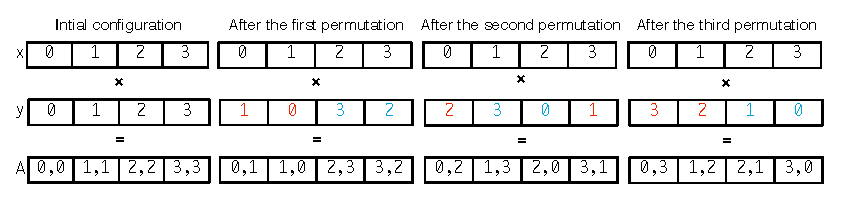
\includegraphics[scale=0.6]{coffee/pictures/vect-by-vect-inline.pdf}}
\caption{Outer-product vectorization by permuting values in a vector register.}
\label{fig:vect-by-vect}
\end{figure}

The storage layout of $A$, however, is incorrect after the application of this outer-product-based vectorization (\emph{op-vect}, in the following). It can be efficiently restored with a sequence of vector shuffles following the pattern highlighted in Figure~\ref{fig:restore-layout}, executed once outside of the \texttt{ijk} loop nest. The pseudo-code for the Burgers local assembly kernel when using \emph{op-vect} is shown in Listing~\ref{code:burgers-opvect}.

\begin{figure}
\centerline{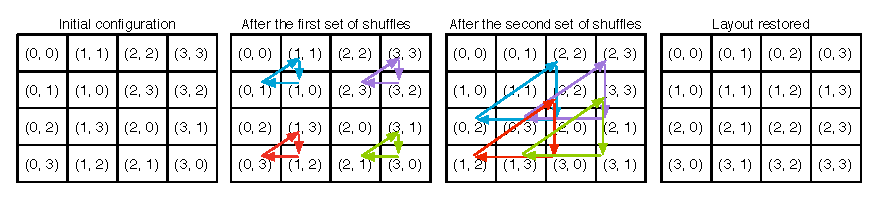
\includegraphics[scale=0.6]{coffee/pictures/vect-restore-inline.pdf}}
\caption{Restoring the storage layout after \emph{op-vect}. The figure shows how 4$\times$4 elements in the top-left block of the element matrix $A$ can be moved to their correct positions. Each rotation, represented by a group of three same-colored arrows, is implemented by a single shuffle intrinsic.}
\label{fig:restore-layout}
\end{figure}


\subsection{Exposing Matrix-Matrix Multiplications for BLAS Operations}
\label{sec:coffee-blas}

In this section, a way of systematically transforming the local element matrix computation into a sequence of matrix-matrix multiplication operations is discussed. 

If such operations could be exposed, highly-optimized dense linear algebra libraries, for instance MKL or ATLAS BLAS, could be used, which would potentially result in notable performance improvements. It is true that the basis functions' size is usually too small to obtain any gain from BLAS routines, which are tuned for large arrays~\citep{nek5000}; however, this can significantly increase with the order of the method and due to the presence of coefficient functions in the equation. Since our research is an exploration of optimization techniques for generic equations (i.e. nothing is assumed about the order of the method and the mathematical structure of the form), an algorithm capable of translating assembly expressions into a sequence of BLAS calls has been studied. The main steps of the algorithm are informally provided next. 

By fully applying the rewrite rules in Figure~\ref{fig:rewrite-rules}, an assembly expression is reduced to a summation, over each quadrature point, of outer products along the test and trial functions. Each outer product is then isolated, i.e. the assembly expression is split into chunks, each chunk representing an outer product over test and trial functions. Statements in the bodies of the surrounding loops (e.g. coefficients evaluation at a quadrature point, temporaries introduced by expression rewriting) are vector-expanded and hoisted completely outside of the loop nest, similarly to what we have described in Section~\ref{sec:coffee-precompute}. This renders the loop nest perfect; that is, there is no intervening code among the various loops. The element matrix evaluation has now become a sequence of dense matrix-matrix multiplies (transposition aside)
\begin{equation*}
A_{jk} = \sum_{i} x_{0_{ij}} \cdot y_{0_{ik}} + \sum_{i} x_{1_{ij}} \cdot y_{1_{ik}} + ...
\end{equation*}
where $x0, x1, y0, y1, ...$ are tabulated basis functions or vector-expanded temporaries introduced at expression rewriting time. Eventually, the storage layout of the involved operands is changed so as to be conforming to the BLAS interface (e.g. two dimensional arrays are flatten as one dimensional arrays). The translation into a sequence of DGEMM calls is the last, straightforward step. 

\section{General-purpose Optimizations}
\label{sec:coffee-genpurp-opts}

\subsection{Loop Interchange}
\label{sec:coffee-genpurp-opts-interchange}
All loops are interchangeable, provided that temporaries are introduced if the nest is not perfect. For the employed storage layout, the loop permutations \texttt{ijk} and \texttt{ikj} are likely to maximize performance. Conceptually, this is motivated by the fact that if the \texttt{i} loop were in an inner position, then a significantly higher number of load instructions would be required at every iteration. We tested this hypothesis in manually crafted kernels. We found that the performance loss is greater than the gain due to the possibility of accumulating increments in a register, rather than memory, along the \texttt{i} loop. The choice between \texttt{ijk} and \texttt{ikj} depends on the number of load instructions that can be hoisted out of the innermost dimension. As discussed in the next sections, a good heuristics it to choose as outermost the loop along which the number of invariant loads is smaller so that more registers remain available to carry out the computation of the local element matrix.

\subsection{Loop Unroll}
Loop unroll (or unroll-and-jam of outer loops) is fundamental to the exposure of instruction-level parallelism, and tuning unroll factors is particularly important.

We first observe that manual full (or extensive) unrolling is unlikely to be effective for two reasons. Firstly, the \texttt{ijk} loop nest would need to be small enough such that the unrolled instructions do not exceed the instruction cache, which is rarely the case: it is true that in a local assembly kernel the minimum size of the \texttt{ijk} loop nest is 3$\times$3$\times$3 (triangular mesh and polynomial order 1), but this increases rapidly with the polynomial order of the method and the discretization employed (e.g. tetrahedral meshes imply larger loop nests than triangular ones), so sizes greater than 10$\times$10$\times$10, for which extensive unrolling would already be harmful, are in practice very common. Secondly, manual unrolling is dangerous because it may compromise compiler auto-vectorization by either removing loops (most compilers search for vectorizable loops) or losing spatial locality within a vector register.

By comparison with implementations characterized by manually-unrolled loops, we noticed that recent versions of compilers like GNU's and Intel's estimate close-to-optimal unroll factors when the loops are affine and their bounds are relatively small and known at compile-time, which is the case of our kernels. Unless an auto-tuning system is used (this option is discussed in Section~\ref{sec:coffee-autotune}) our choice is to leave the backend compiler in charge of applying loop unroll. 

%TODO: maybe we can clarify that unroll-and-jam for opvect corresponds to changing the tile size...

\section{COFFEE: an Optimizing Compiler for Finite Element Local Assembly}
\label{sec:coffee-implementation}
\subsection{Outline and Integration with Firedrake}

\begin{figure}
\begin{center}
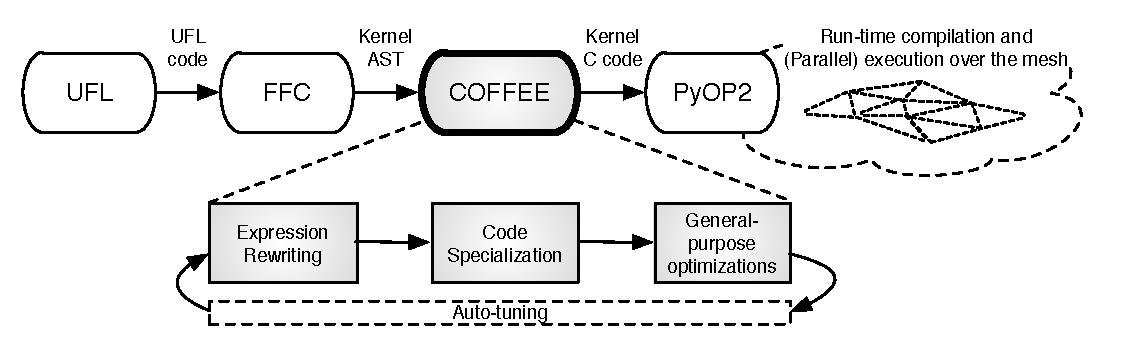
\includegraphics[scale=0.70]{coffee/pictures/coffee-pipeline.pdf}
\caption{High-level view of Firedrake. COFFEE is at the core, receiving ASTs from a modified version of the FEniCS Form Compiler and producing optimized C code kernels.}
\label{fig:coffee-pipeline}
\end{center}
\end{figure}

Our research resulted in the implementation of COFFEE\footnote{COFFEE stands for COmpiler For FinitE Element local assembly.}, a mature, platform-independent compiler capable of optimizing any local assembly code generated through Firedrake or FEniCS. COFFEE has been fully integrated with Firedrake, so it can optimize any equation expressible with this framework. The code, which comprises more than 5000 lines, is available at~\citep{coffee-implementation}.

Firedrake users employ the Unified Form Language to express problems in a notation resembling mathematical equations. At run-time, the high-level specification is translated by a modified version of its form compiler, the FEniCS Form Compiler (FFC)~\cite{FFC-Compiler}, into an abstract syntax tree (AST) representation of one or more finite element assembly kernels. ASTs are then passed to COFFEE to apply the transformations described in the previous sections. The output of COFFEE, C code, is eventually provided to PyOP2~\citep{pyop2isc}, where just-in-time compilation and execution over the discretized domain take place. The flow and the compiler structure are outlined in Figure~\ref{fig:coffee-pipeline}. 

The compiler applies an ordered sequence of optimization steps to the ASTs received from FFC. Expression rewriting is performed first, due to the introduction of temporary arrays and the need to create multiple loop nest starting from the original one (this may happen when computation over zero-valued blocks is avoided). Then, code specialization takes place. Finally, loop interchange and loop unroll are applied. COFFEE has an auto-tuning system, described in Section~\ref{sec:coffee-autotune}, to individuate the most suitable optimization strategy (i.e. to select which transformations to apply) for a certain equation. The implementation of all code transformations is centered on analysis and manipulation of the kernel AST. Any possible corner cases are handled: for example, if outer-product vectorization is to be applied but the size of the iteration space is not a multiple of the vector length, then a remainder loop, amenable to auto-vectorization, is inserted (as shown in Figure~\ref{code:burgers-opvect}).

Users can either enable individual transformations by switching specific flags or leave the auto-tuning system, described in Section~\ref{sec:coffee-autotune}, in charge of determining the best optimization strategy (i.e. selecting and composing transformations).

\subsection{Modifying the FEniCS Form Compiler}
COFFEE expects as input either a string of C code or an AST. In the former case, a parser could be used to obtain an AST representation, which is required by the algorithms implementing the various code transformations. Therefore, FFC's output, which is a C-code implementation of a local assembly kernel, could be used straightforwardly as input to COFFEE. However, we note that this would also be conceptually pointless: FFC would generate C code from its intermediate representation that eventually COFFEE would have to re-parse to obtain an AST. A much cleaner solution, adopted and explained next, consists of modifying FFC to directly generate an AST. 

\subsubsection{Generation of Abstract Syntax Trees}
The construction of the FFC's intermediate representation from UFL code is refined as follows:
\begin{itemize}
\item The mathematical expression that evaluates the element matrix is represented by a tree data structure. A limitation of the original FFC was that nodes in such expression tree, which correspond to symbols or arithmetic operations, are not bound to the enclosing loops. For instance, consider the symbol \texttt{A[i][j]}: the FFC's expression tree has a node for this symbol, but visiting it there is no clean way of separating the variable name \texttt{A} from the loop indices \texttt{i} and \texttt{j}. Therefore, we have enriched symbol nodes with additional fields to capture these information. 
\item Basis functions in the FFC's intermediate representation are characterized by a new field telling whether they originated from a vector-valued or a scalar-valued element. In the former case, the array rappresenting the tabulation of a basis function at the various quadrature points is block-sparse. This information is recorded and, as explained next, attached to the kernel's AST to enable COFFEE applying symbolic execution to avoid iteration over zero-valued blocks, as elaborated in Section~\ref{sec:coffee-avoidzeros}.
\end{itemize}
To make FFC output ASTs, its intermediate representation is intercepted prior to the code generation stage and forwarded to a new module, which is referred to as \texttt{ast-generation}. The structure of the modified version of FFC is illustrated in Figure~\ref{fig:coffee-ffc}. The \texttt{ast-generation} stage ``mirrors'' the actions of code generation, but it differs by rather building an AST. An example is provided in Figure~\ref{fig:coffee-ast-vs-c}. To achieve this, COFFEE exposes its hierarchy of AST nodes, which are suitably instantiated and composed in \texttt{ast-generation}. 

The enriched intermediate representation allows to create proper AST's Symbol nodes. A Symbol, as shown in Figure~\ref{fig:coffee-ast-vs-c}, has a name (the variable name), an array of indices, and an array of offsets. These information are fundamental for the implementation of expression rewriting and code specialization. Further, special AST's Declaration objects can be used to track the sparsity pattern in basis function arrays. 

\subsection{On the Compiler Implementation}
Figure~\ref{fig:coffee-compiler-structure} outlines the various modules composing COFFEE. Expression rewriting, code specialization, and general-purpose transformations are applied by manipulating the AST representing the local assembly kernel. Providing the steps of all algorithms performing the various transformations would just be tedious and marginally helpful for the reader; essentially, implementing a transformation always reduces to write a routine that visits and manipulates a tree data structure (the AST) according to the semantics described in Sections~\ref{sec:coffee-expr-rewrite} and~\ref{sec:coffee-code-spec}. In this section, we rather focus on aspects of the compiler implementation that involve the orchestration of the different transformations, including a description of the data structures employed to track both the restructuring of the assembly expressions and data dependencies. 

\subsubsection{Code Hoisting}
Hoisting is the operation of moving code, for instance a statement or the evaluation of an expression, from an inner to an outer loop in a nest. This operation is performed in several occasions when rewriting an expression: generalized loop-invariant code motion, expansion of sub-expressions, and precomputation of terms all require code hoisting, as illustrated in Figures~\ref{code:invariant-code} and~\ref{code:expanded-code}. In order to perform code hoisting, in particular, several aspects must be known:
\begin{enumerate}
\item ``what'' to hoist
\item ``where'' to hoist (possibly, outside of the loop nest)
\item if scalar-expansion should be introduced
\end{enumerate}
Answers to these three points obviously depend on the specific transformation, although parts of the implementation are shared. COFFEE tracks hoisted code by means of a dictionary that binds variable names (guaranteed to be unique) to a set of information. In particular, for a variable \texttt{v}, the dictionary provides:
\begin{itemize}
\item a reference to the AST node corresponding to the expression \texttt{e} hosted by \texttt{v};
\item a reference to the loop in which \texttt{v} is assigned \texttt{e};
\item a reference to the AST node corresponding to the declaration of \texttt{v}.
\end{itemize}
As expressions are hoisted, the dictionary is populated and/or updated with new information. For example, when applying generalized loop-invariant code motion, a new entry is created, unless the sub-expression being lifted has already been pre-computed elsewhere. On the other hand, when sub-expressions are expanded, either a new entry is created or an old entry is updated, as explained in Section~\ref{sec:coffee-expansion}. 

The dictionary is also queried at code specialization time for padding, data alignment and generation of BLAS calls. Therefore, different algorithms in COFFEE access the same data structure, which allows avoiding both duplicated code and an additional overhead due to revisiting the same portion of AST in distinct transformations.

\subsubsection{Benefits of Tracking Data Dependencies}
COFFEE implements ``smart'' code hoisting: everytime a sub-expression or a term are lifted, for example from the mathematical expression evaluating the local element matrix to an outer level in the loop nest, three optimizations are potentially applied. Consider a hoistable expression \texttt{e} assuming different values in the iteration space \texttt{I}:
\begin{itemize}
\item \textbf{Minimize redundant computation.} If an equivalent sub-expression \texttt{e'} has already been hoisted along the iteration space \texttt{I}, then COFFEE replaces \texttt{e} with a reference to the symbol hosting the value of \texttt{e'}. This avoids both redundant computation and the introduction of additional temporary variables;
\item \textbf{Loop fusion.} If scalar-expansion is introduced (we recall this is useful to achieve SIMD auto-vectorization; see Sections~\ref{sec:coffee-licm} and~\ref{sec:coffee-precompute}), then the hoisted code must be placed in an outer loop \texttt{r}, \texttt{r $\in$ I}. This was the purpose of the second \texttt{r} loop in Figure~\ref{code:invariant-code}; note that this loop includes scalar-expanded sub-expressions that, in the non-transformed code, iterated along logically different spaces (loops \texttt{j} and \texttt{k}, corresponding to test and trial functions). In this example, it was possible to use a single \texttt{r} loop because we assumed that test and trial function spaces were the same, leading to identical loop bounds; in general, however, this is not true. Another assumption of the example was that the space of the equation's coefficients (variables \texttt{f0, f1} in the figure) coincided with that of test and trial functions. This would allow fusing the two \texttt{r} loops, which is exactly what COFFEE does, although not displayed by the figure. Fusing loops, which increases data locality and reduces loop overhead, is possible in some circumnstances, in particular when there are no data dependencies among hoisted expressions and the spaces of test, trial, and coefficent functions are identical. As explained next, COFFEE reasons about data dependencies and iteration spaces to determine the safeness of loop fusion.
\item \textbf{Reduce extra memory.} When expanding an expression, terms hoisting is possible to relieve register pressure. This poses the challenge described in Section~\ref{sec:coffee-expansion} and intuitively summarized in Figure~\ref{code:expanded-code}; that is, understanding whether it is possible to absorb the hoistable term in an available temporary value or a new temporary is needed. Obviously, the less is the number of temporaries introduced, the smaller is the size of the working set, which may result in better performance.
\end{itemize}
To implement these optimizations, it is necessary to track the evolution of data dependencies as the assembly expression is rewritten. For this purpose, COFFEE uses a dependency graph, which is a standard approach used by general-purpose compilers relying on abstract syntax trees (in addition to other data structures) as intermediate representation. The dependency graph has as many nodes as the number of variables in the loop nest characterizing the assembly expression. A direct edge from a node \texttt{A} to a node \texttt{B} indicates that the value of symbol \texttt{B} depends on that of \texttt{A}. 

The implementation of the depedency graph data structure and of the various algorithms using it is made simple by the fact that COFFEE ensures \textit{static single assignment} form. This property, typically adopted by intermediate representations in compilers, requires that variables are assigned exactly once, and that each variable is defined in advance. 

\subsubsection{Specialization}


\subsection{Model-driven Dynamic Autotuning}
\label{sec:coffee-autotune}

Determining the sequence of transformations that maximizes the performance of a problem requires investigating a broad range of factors, including mathematical structure of the input form, polynomial order of employed function spaces, presence of pre-multiplying functions, and, of course, the characteristics of the underlying architecture. The set of possible optimizations is very large, so the selection problem is challenging. The sole Expression Rewriter, for instance, can generate a wide variety of implementations by just applying rewrite rules up to different extents.  

We tackle the optimizations selection problem by compiler autotuning. Not only does it allow to determine the best combination of transformations, also it enables exploring parametric low-level optimizations, such as loop unroll, unroll-and-jam, and interchange, by trying different unroll factors and loop permutations. By leveraging domain knowledge and a set of heuristics, we manage to keep the autotuner overhead to a minimum, whilst achieving significant speed ups over a fixed optimization strategy, as shown in Section~\ref{sec:coffee-allforms-perf}. In particular, our autotuner usually requires order of seconds to determine the fastest kernel implementation, a negligible overhead when it comes to iterate over real-life unstructured meshes; details will be provided later.

COFFEE analyzes the input problem and decides what variants it is worth testing through autotuning, as described later. Each variant is obtained by requesting specific transformations to the Expression Rewriter and the Code Specializer. The possible variants are then provided to the autotuner, in the form of abstract syntax trees. The autotuner is a template-based code generator. By inspecting an abstract syntax tree, it determines how to generate ``wrapping'' code that 1) initializes kernel's input variables with fictitious values and 2) calls the kernel. These two points are executed repeatedly in a \emph{while} loop for a pre-established amount of time (order of milliseconds). At the exit of the \emph{while} loop, the times the kernel was invoked is recorded. Eventually, the variant executed the largest number of iterations is designated as the fastest implementation. Suitable compiler directives are used to prevent inlining of all function calls: this avoids the situation in which some variants are inlined and some are not, which would fake the autotuner's output. 

The autotuning process is dynamic: depending on the complexity of the input problem, more or less variants are tried. General heuristics, which can be considered a revisited version of those presented in~\cite{nek5000}, are applied:
\begin{itemize}
\item Loop permutations that are likely to worsen the performance are excluded from the search space. According to what explained in Section~\ref{sec:coffee-genpurp-opts-interchange}, we enable only variants in which the loop over quadrature points is either the outermost or the innermost. This is due to the fact that versions of the code in which such loop lies between the test and trial functions loops are typically lower performing.
\item The unroll factors must divide the loop bounds evenly to avoid the introduction of reminder (scalar) loops.
\item The innermost loop is never explicitly unrolled. This is because we expect auto-vectorization along this loop, so memory accesses should be kept unit-stride. 
\item Padding and data alignment are always applied. 
\end{itemize}
The auto-tuning system is domain-aware; that is, it exploits the following heuristics, which capture properties of the computational domain:
\begin{itemize}
\item The length of test and trial functions loops are identical in some cases, for example when they originate from the same function space. In such cases, since for the employed storage layout the memory access pattern is symmetrical along these two loops, we prune their interchange from the search space. 
\item The larger is the polynomial order of the method, the larger is the assembly loop nest. In these cases, we impose a bound on the loop nest's overall unroll factor (which we found empirically) to avoid uselessly testing too many unroll factors. 
\item On the other hand, if the polynomial order is low, i.e. when the loop nest is small, we prune variants that we know will be low-performing, e.g. those resorting to BLAS.
\item We specifically select two levels of expression rewriting. In the ``base'' level, only generalized loop-invariant code motion is applied. This means that only a subset of the rewrite rules exposed in Section~\ref{fig:rewrite-rules} will be considered. In the ``aggressive'' level, all of the rewrite rules are applied, which means terms factorization, precomputation, and expansion (Sections~\ref{sec:coffee-factorize}-\ref{sec:coffee-expansion}) are introduced. Many other trade-offs, which we do not explore, would be feasibile, however. 
\item For the expression splitting optimization described in Section~\ref{sec:coffee-split}, only three split factors are tested, namely 1, 2, 4. Also, if the input problem uses vector-valued function spaces, the iteration space is already split at expression rewriting time to avoid computation over zero-valued columns; in such a case, we do not further apply expression splitting.
\end{itemize}

All of the previous points contribute to minimize the overhead of the autotuning process. We will discuss the actual cost of autotuning in Section~\ref{sec:coffee-pereval-autotune}.

\section{Performance Analysis}
\label{sec:coffee-perfeval}

\subsection{Experimental Setup}
\label{sec:coffee-perfeval-setup}
Experiments were run on a single core of an Intel architecture, a Sandy Bridge I7-2600 CPU running at 3.4GHz, with 32KB of L1 cache and 256KB of L2 cache). The \texttt{icc 14.1}  compiler was used. On the Sandy Bridge, the compilation flags used were \texttt{-O2} and \texttt{-xAVX} for auto-vectorization. Other optimization levels performed, in general, slightly worse.

Three studies are presented. Firstly, in Section~\ref{sec:coffee-perfeval-single}, the impact of individual code transformations is analyzed in three real-world,
representative equations. We believe it is important to clarify \textit{in which contexts} and \textit{why} such optimizations can provide speed ups. Secondly, we show that combining aggressive expression rewriting and code specialization allows outperforming both (i) a basic optimization strategy (where only a few of COFFEE's transformations are enabled) and (ii) the FEniCS Form Compiler's built-in optimization system. Experiments are carried out in a set of notable equations. In these first two studies, the speedups achievable at the level of the local assembly kernel are quantified; that is, the other stages of the computation (e.g. global assembly, problem setup) are excluded from the measurements. Finally, in Section~\ref{sec:coffee-pereval-fullapp}, a full application investigation is provided to demonstrate that our techniques for cross-loop optimization of arithmetic intensity allow a significant reduction in the overall computation run-time to be achieved, which ultimately demonstrates the success of our research.

\subsection{Contribution of Individual Optimizations}
\label{sec:coffee-perfeval-single}

\subsubsection{Rationale of the Study}
\label{sec:coffee-individual-rationale}
We evaluate some critical code transformations in three real-world problems based on the following PDEs: (i) Helmholtz, (ii) Diffusion, and (iii) Burgers. The evaluation concerns:
\begin{itemize}
\item Generalized loop-invariant code motion (Section~\ref{sec:coffee-licm})
\item Padding and data alignment (Section~\ref{sec:coffee-padding})
\item Expression splitting (Section~\ref{sec:coffee-split})
\item Vector-register tiling (Section~\ref{sec:coffee-opvect})
\end{itemize}
\textit{The goal of this section is to demonstrate the effectiveness of individual transformations and to explain under what circumnstances performance improvements are obtainable}. It is important to understand \textit{for what reasons} gains in run-time are achieved with these critical optimizations; some transformations are excluded from this study for reasons of time and readability of the section, but analogous considerations and observations would apply. 
%However, in Section~\ref{sec:coffee-perfeval-allforms}, we will show that an aggressive optimization strategy based on extensive expression rewriting, code specialization, and exploitation of COFFEE's auto-tuning system can outperform the cumulative impact of the transformations analyzed in the present section.

The three chosen equations are \emph{real-life kernels} and comprise the core differential operators in some of the most frequently encountered finite element problems in scientific computing. This is of crucial importance because distinct problems, possibly arising in completely different fields, may employ (subsets of) the same differential operators of our benchmarks, which implies similarities and redundant patterns in the generated code. Consequently, the proposed code transformations have a domain of applicability that goes far beyond that of the three analyzed equations.

The Helmholtz and Diffusion kernels are archetypal second order elliptic operators. They are complete and unsimplified examples of the operators used to model diffusion and viscosity in fluids, and for imposing pressure in compressible fluids. As such, they are both extensively used in climate and ocean modeling. Very similar operators, for which the same optimisations are expected to be equally effective, apply to elasticity problems, which are at the base of computational structural mechanics. The Burgers kernel is a typical example of a first order hyperbolic conservation law, which occurs in real applications whenever a quantity is transported by a fluid (the momentum itself, in our case). We chose this particular kernel since it applies to a vector-valued quantity, while the elliptic operators apply to scalar quantities; this impacts the generated code, as explained next. The operators we have selected are characteristic of both the second and first order operators that dominate fluids and solids simulations.
%and a wide variety on local assembly codes can be tested.

The benchmarks were written in UFL (code available at~\cite{ufl-code}) and executed over real unstructured meshes through Firedrake. The Helmholtz code has already been shown in Listing~\ref{code:helmholtz}. The Diffusion equation uses the same differential operators as Helmholtz. In the Diffusion kernel code, the main differences with respect to Helmholtz are the absence of the $Y$ array and the presence of additional constants for computing the element matrix. Burgers is a non-linear problem employing differential operators different from those of Helmholtz and relying on vector-valued quantities, which has a major impact on the generated assembly code (see Listing~\ref{code:burgers}), where a larger number of basis function arrays ($X1$, $X2$, ...) and constants ($F0$, $F1$, ..., $K0$, $K1$,
...) are generated. 

These problems were studied varying both the shape of mesh elements and the polynomial order $q$ of the method, whereas the element family, Lagrange, is fixed. As might be expected, the larger the element shape and $q$, the larger the iteration space. Triangles, tetrahedra, and prisms were tested as element shape. For instance, in the case of Helmholtz with $q=1$, the size of the \texttt{j} and \texttt{k} loops for the three element shapes is, respectively, $3$, $4$, and $6$. Moving to bigger shapes has the effect of increasing the number of basis function arrays, since, intuitively, the behaviour of the equation has to be approximated also along a third axis. On the other hand, the polynomial order affects only the problem size (the three loops \texttt{i}, \texttt{j}, and \texttt{k}, and, as a consequence, the size of $X$ and $Y$ arrays). A range of polynomial orders from $q=1$ to $q=4$ were tested; higher polynomial orders are excluded from the study because of current Firedrake limitations. In all these cases, the size of the element matrix rarely exceeds 30$\times$30, with a peak of 105$\times$105 in Burgers with prisms and $q=4$.

\begin{figure}[t]
\centerline{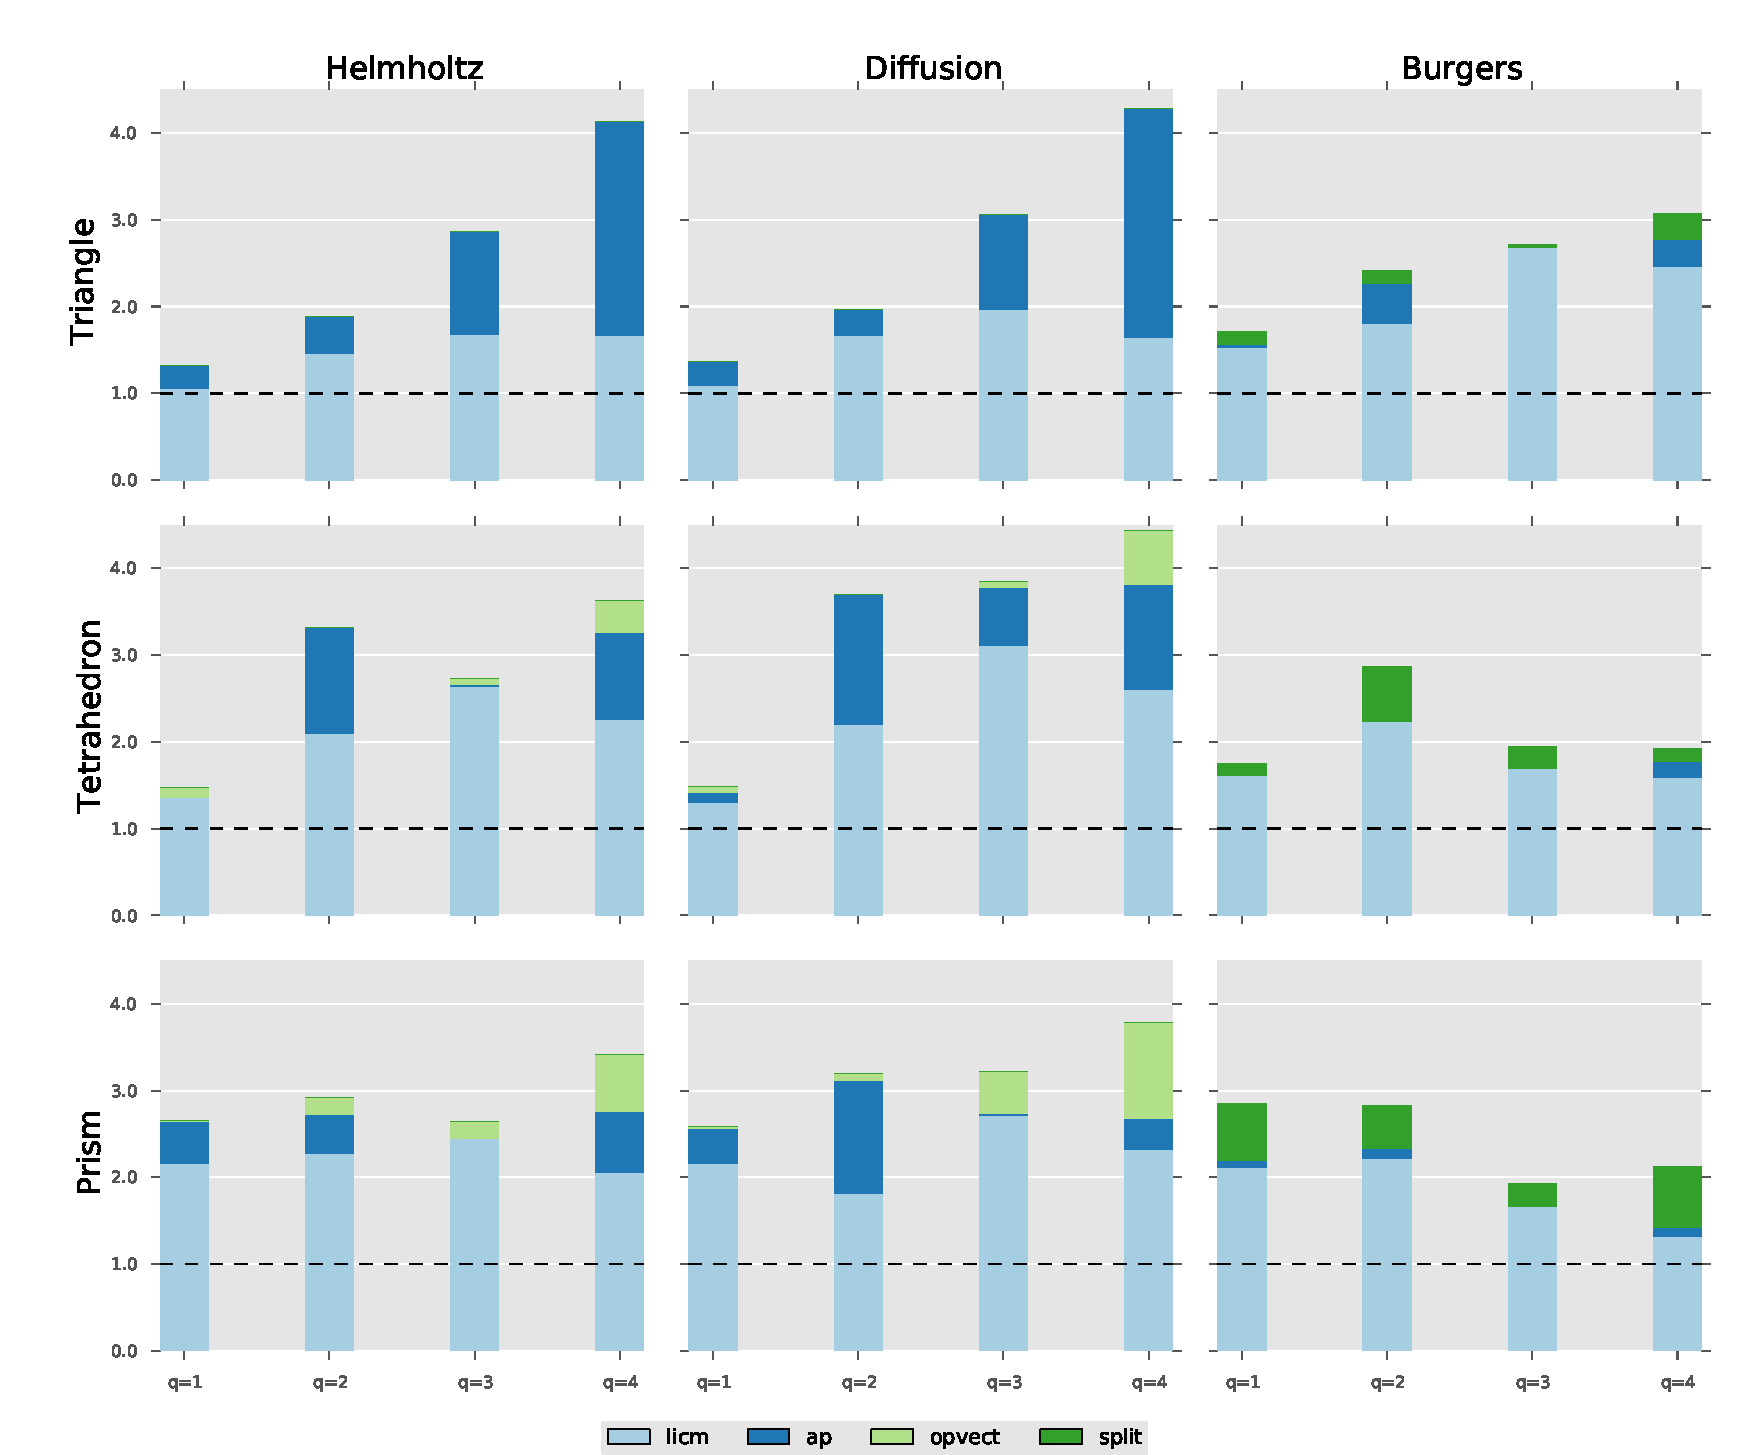
\includegraphics[scale=0.45]{coffee/perf-results/individual/graph}}
\caption{Performance improvement due to generalized loop-invariant code motion (\emph{licm}), data alignment and padding (\emph{ap}), outer-product vectorization (\emph{op-vect}), and expression splitting (\emph{split}) over the original non-optimized code. In each plot, the horizontal axis reports speed ups, whereas the polynomial order $q$ of the method varies along the vertical axis.}
\label{fig:coffee-individual-res}
\end{figure}

The speed ups due to applying optimizations over the original local assembly code are shown in Figure~\ref{fig:coffee-individual-res}. The figure itself can be read as a ``plot of plots'': the various element shapes are reported on the horizontal axis, whereas each equation corresponds to one point along the vertical axis. This allows to deduct the behaviour of transformations when varying the parameters of our study in an unified way. In the next sections, we refer to this figure and elaborate on the impact of individual transformations. We shorten generalized loop-invariant code motion as \emph{licm}; padding and data alignment as \emph{ap}; outer-product vectorization as \emph{op-vect}; expression splitting as \emph{split}.

\subsubsection{Impact of Generalized Loop-invariant Code Motion}
\label{sec:perf-eval-licm}

In general, the speedups achieved by \emph{licm} are notable. The main reasons were anticipated in Section~\ref{sec:coffee-licm}: in the original code, 1) sub-expressions invariant to outer loops are not automatically hoisted, while 2) sub-expressions invariant to the innermost loop are hoisted, but their execution is not auto-vectorized. These observations come from inspection of assembly code generated by the compiler.

The gain tends to grow with the computational cost of the kernels: bigger loop nests (i.e., larger element shapes and polynomial orders) usually benefit from the reduction in redundant computation, even though extra memory for the temporary arrays is required. Some discrepancies to this trend are due to a less effective auto-vectorization. For instance, on the Sandy Bridge, the improvement at $q=3$ is larger than that at $q=4$ because, in the latter case, the size of the innermost loop is not a multiple of the vector length, and a remainder scalar loop is introduced at compile time. Since the loop nest is small, the cost of executing the extra scalar iterations can have a significant impact.

\subsubsection{Impact of Padding and Data Alignment}
\label{sec:perf-eval-padding}

Padding, which avoids the introduction of a remainder loop as described in Section~\ref{sec:coffee-padding}, as well as data alignment, enhance the quality of auto-vectorization. Occasionally the impact of \emph{ap} is marginal. These may be due to two reasons: (i) the non-padded element matrix size is already a multiple of the vector length; (ii) the number of aligned temporaries introduced by \emph{licm} is so large to induce cache associativity conflicts (e.g. Burgers equation).

\subsubsection{Impact of Vector-register Tiling}
\label{sec:perf-eval-opvect}

In this section, we evaluate the impact of vector-register tiling. \emph{op-vect} requires the unroll-and-jam factor to be explicitly set. Here, we report the best speed-up obtained after all feasible unroll-and-jam factors were tried. 

The rationale behind these results is that the effect of \emph{op-vect} is significant in problems in which the assembly loop nest is relatively big. When the loops are short, since the number of arrays accessed at every loop iteration is rather small (between 4 and 8 temporaries, plus the element matrix itself), there is no need for
vector-register tiling; extensive unrolling is sufficient to improve register re-use and, therefore, to maximize the performance. However, as the iteration space becomes larger, \emph{op-vect} leads to improvements up to 1.4$\times$ (Diffusion, prismatic mesh, $q=4$ - increasing the overall speed up from 2.69$\times$ to 3.87$\times$).

Using the Intel Architecture Code Analyzer tool~\cite{IACA}, we confirmed that speed ups are a consequence of increased register re-use. In Helmholtz $q=4$, for example, the tool showed that when using \emph{op-vect} the number of clock cycles to execute one iteration of the \texttt{j} loop decreases by roughly 17$\%$, and that this is a result of the relieved pressure on both of the data (cache) ports available in the core.

The performance of individual kernels in terms of floating-point operations per second was also measured. The theoretical peak on a single core, with the Intel Turbo Boost technology activated, is 30.4 GFlop/s. In the case of Diffusion using a prismatic mesh and $q=4$, we achieved a maximum of 21.9 GFlop/s with \emph{op-vect} enabled, whereas 16.4 GFlop/s was obtained when only \emph{licm-ap} is used. This result is in line with the expectations: analysis of assembly code showed that, in the \texttt{jk} loop nest, which in this problem represents the bulk of the computation, 73$\%$ of instructions are actually floating-point operations.

Application of \emph{op-vect} to the Burgers problem induces significant slowdowns due to the large number of temporary arrays that need to be tiled, which exceeds the available logical registers on the underlying architecture. Expression splitting can be used in combination with \emph{op-vect} to alleviate this issue; this is discussed in the next section.

%for which efficient register allocation can be already guaranteed

\subsubsection{Impact of Expression Splitting}
\label{sec:perf-results-split} 
Expression splitting relieves the register pressure when the element matrix evaluation needs to read from a large number of basis function arrays. As detailed in Section~\ref{sec:coffee-split}, the price to pay for this optimazion is an increased number of accesses to the element matrix and, potentially, redundant computation. 

For the Helmholtz and Diffusion kernels, in which only between 4 and 8 temporaries are read at every loop iteration, \texttt{split} tends to slow down the computation, because of the aforementioned drawbacks. Slow downs up to 1.4$\times$ were observed. 

In the Burgers kernels, between 12 and 24 temporaries are accessed at every loop iteration, so \emph{split} plays a key role since the number of available logical registers on the Sandy Bridge architecture is only 16. In almost all cases, a split factor of 1, meaning that the original expression was divided into two parts, ensured close-to-peak perforance. The transformation negligibly affected register locality, so speed ups up to 1.5$\times$ were observed. For instance, when $q=4$ and a prismatic mesh is employed, the overall performance improvement increases from 1.44$\times$ to 2.11$\times$. 

The performance of the Burgers kernel on a prismatic mesh was 20.0 GFlop/s from $q=1$ to $q=3$, while it was 21.3 GFlop/s in the case of $q=4$. These values are notably close to the peak performance of 30.4 GFlop/s. Disabling \emph{split} makes the performance drop to 17.0 GFlop/s for $q=1, 2$, 18.2 GFlop/s for $q=3$,
and 14.3 GFlop/s for $q=4$. These values are in line with the speedups shown in Figure~\ref{fig:coffee-individual-res}.

The \emph{split} transformation was also tried in combination with \emph{op-vect} (\emph{split-op-vect}). Despite improvements up to 1.22$\times$, \emph{split-op-vect} never outperforms \emph{split}. This is motivated by two factors: for small split factors, such as 1 and 2, the data space to be tiled is still too big, and register spilling affects run-time; for higher ones, sub-expressions become so small that, as explained in Section~\ref{sec:perf-eval-opvect}, extensive unrolling already allows to achieve a certain degree of register re-use.

\subsubsection*{Results on Other Architectures}
To avoid impairing the readability of the section, which already contains a vast amount of information, we are not reporting performance results on the Intel Xeon Phi  architecture (each core running at 1.05Ghz in native mode, 32KB L1 cache and 512KB L2 cache). With respect to the Sandy Bridge, this architecture has a different number of logical registers and SIMD lanes (16 256-bit registers in the Sandy Bridge, and 32 512-bit registers in the Xeon Phi), which can impact the optimization strategy. The interested reader is invited to refer to the published paper~\citep{Luporini-coffee}.

\subsection{Evaluation in Forms of Increasing Complexity}
\label{sec:coffee-perfeval-allforms}

\subsubsection{Rationale of the Study}
\label{sec:coffee-allforms-rationale}
We analyze the run-time performance of four fundamental real-world problems, which comprise the differential operators that are most common in finite element methods. In particular, our study includes problems based upon the Helmholtz and Poisson equations, as well as elasticity- and hyperelasticity-like forms. The Unified Form Language~\cite{ufl} specification for these forms, which is the domain specific language that both Firedrake and FEniCS use to express weak variational form, is available at~\cite{ufl-code}. 

We evaluate the \textit{speed ups} achieved by three sets of optimizations over the original code; that is, the code generated by the FEniCS Form Compiler when no optimizations are applied. In particular, we analyze the impact of the FEniCS Form Compiler's built-in optimizations (henceforth \texttt{ffc}), the impact of COFFEE's transformations as presented in Section~\ref{sec:coffee-perfeval-single} (referred to as \texttt{fix}, in the following), and the impact due to COFFEE auto-tuning expression rewriting and code specialization (henceforth \texttt{auto}, to denote the use of autotuning). The \texttt{auto} values do not include the auto-tuning overhead, which is commented aside in Section~\ref{sec:coffee-pereval-autotune}. All codes were executed in the context of the Firedrake framework.

%This way, we also highlight the advances achieved over our previous work. 
%...TODO...: dire che i tempi sono la media di 3 runs

The values that we report include the cost of local assembly as well as the cost of matrix insertion. However, the (unstructured) mesh was made small enough to fit the L3 cache of the architecture, so as to minimize the overhead due to any operations that are not part of the element matrix evaluation itself. We also reinforce the concept that the cost of local assembly becomes increasingly dominant in the whole finite element calculation as the complexity of the form increseas (e.g.~\citep{quadrature-olegaard}). 

We do not compare to the FEniCS Form Compiler's tensor contraction mode~\citep{tensor-kirby} because of three reasons: first, in~\citep{quadrature-olegaard} it has been demonstrated the superiority of quadrature as the complexity of a form increases, so it would be superfluous to repeat the same analysis. Second, our aim is to show the effect of low-level optimizations on the code, especially SIMD vectorization, which is not feasible in tensor mode due to the inherent structure of the code. Third, tensor mode code generation fails due to hardware limitations in many of the test cases that we show below.

We vary several aspects of each form, which follows the approach and the notation of~\citep{quadrature-olegaard} and~\citep{francis}
\begin{itemize}
\item The polynomial order of basis functions, $q \in \lbrace1, 2, 3, 4\rbrace$
\item The polynomial order of coefficient (or ``pre-multiplying'') functions, $p \in \lbrace1, 2, 3, 4\rbrace$
\item The number of coefficient functions $nf \in \lbrace0, 1, 2, 3\rbrace$
\end{itemize}
On the other hand, other aspects are fixed 
\begin{itemize}
\item The space of both basis and coefficient functions is Lagrange
\item The mesh is three-dimensional, made of tetrahedrons, for a total of 4374 cells
\end{itemize}

Figures~\ref{fig:coffee-allforms-helmholtz},~\ref{fig:coffee-allforms-elasticity},~\ref{fig:coffee-allforms-poisson}, and~\ref{fig:coffee-allforms-hyperelasticity}, which will be deeply commented in the next sections, must be read as ``plots, or grids, of plots''. Each grid (figure) has two logical axes: $p$ varies along the horizontal axis, while $q$ varies along the vertical axis. The top-left plot in a grid shows speed ups for $[q=1, p=1]$; the plot on its right does the same for $[q=1, p=2]$, and so on. The diagonal of the grid shows plots for which basis and coefficient functions have same polynomial order, that is $q=p$. Therefore, a grid can be read in many different ways, which allows us to make structured considerations on the effect of the various optimizations. 

A plot reports speed-ups over non-optimized FEniCS-Form-Compiler-generated code. There are three groups of bars, each group referring to a particular version of the code (\texttt{ffc, fix, auto}). There are four bars per group: the leftmost bar corresponds to the case $nf = 0$, the one on its right to the case $nf = 1$, and so on. 

\subsection{Results of General Applicability}
\label{sec:coffee-allforms-perf}
The four chosen forms allow us to perform an in-depth evaluation of different classes of optimizations for local assembly. We limit ourselves to analyzing the cost of computing element matrices, although all of the techniques presented in this paper are immediately extendible to the evaluation of local vectors. As anticipated, in the following we comment speed ups of \texttt{ffc}, \texttt{fix}, and \texttt{auto} over the non-optimized, FEniCS-Form-Compiler-generated code. 

We first comment on results of general applicability. By looking at the various figures, we note there is a trend in the optimizations to become more and more effective as $q$, $p$, and $nf$ increase. This is because most of the transformations applied aim at optimizing for arithmetic intensity and SIMD vectorization, which obviously have a strong impact when arrays and iteration spaces are large. The corner cases of this phenomenon are indeed $[q=1, p=1]$ and $[q=4, p=4]$. We also observe how \texttt{auto}, in almost all scenarios, outperforms all of the other variants. In particular, it is not a surprise that \texttt{auto} is faster than \texttt{fix}, since \texttt{fix} is one of the autotuner's tested variants, as explained in Section~\ref{sec:coffee-autotune}. The reasons for which \texttt{auto} exceeds both original code and \texttt{ffc} are discussed for each specific problem next. Also, details on the ``optimal'' code variant determined by autotuning are given in Section~\ref{sec:coffee-pereval-autotune}.

\subsection{Performance of Helmholtz}
\begin{figure}[t]
\centerline{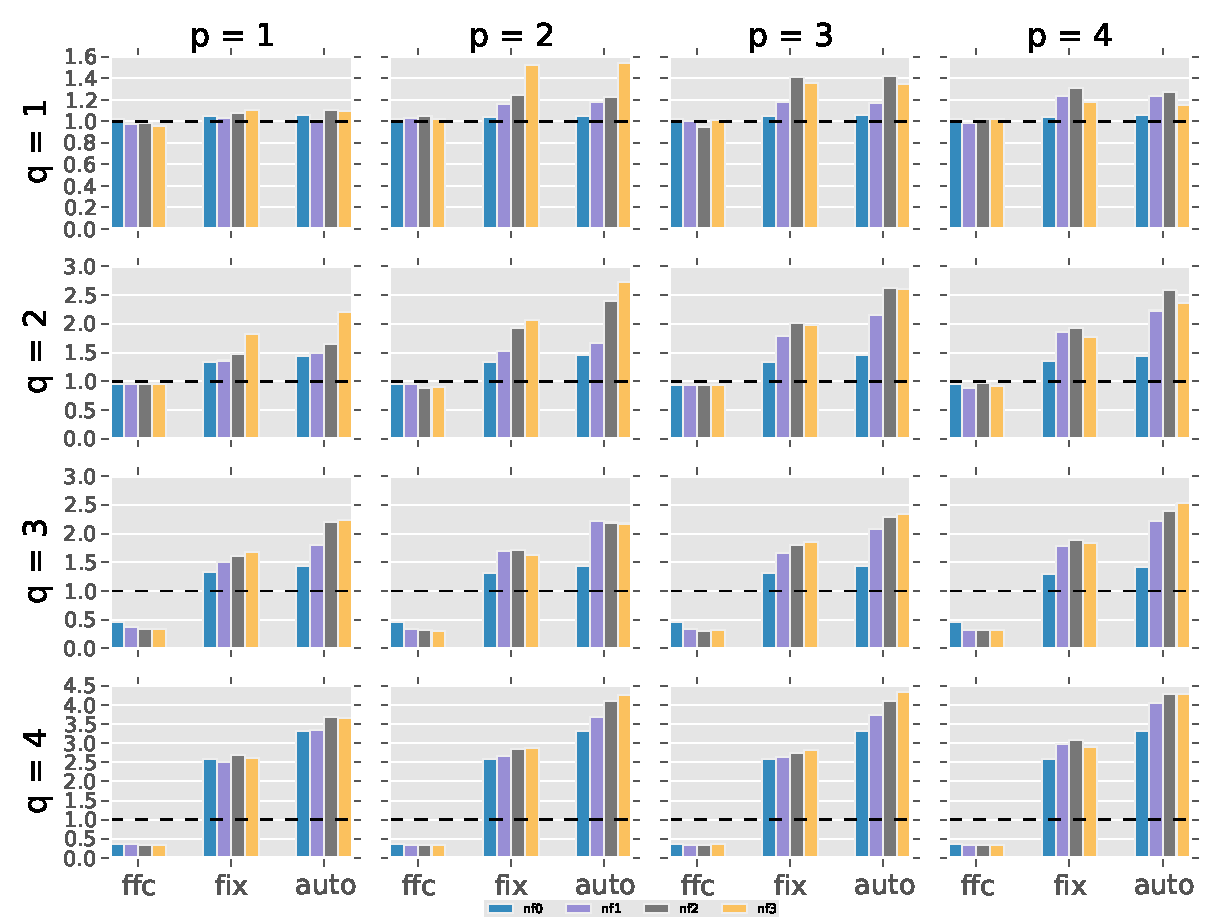
\includegraphics[scale=0.7]{coffee/perf-results/allforms/helmholtz}}
\caption{Helmholtz results.}\label{fig:coffee-allforms-helmholtz}
\end{figure}
The results for the Helmholtz problem are provided in Figure~\ref{fig:coffee-allforms-helmholtz}. We observe that \texttt{ffc} slows the code down, especially for $q \geq 3$. This is a consequence of using indirection arrays in the generated code that, as explained in Section~\ref{sec:coffee-avoidzeros}, prevent, among the other compiler's optimizations, SIMD auto-vectorization. The \texttt{auto} version results in minimal performance improvements over \texttt{fix} when $nf=0$, unless $q=4$. This is due to the fact that if the loop over quadrature points is relatively small, then close-to-peak performance is obtainable through basic expression rewriting and code specialization; in this circumstance, generalized loop-invariant code motion and padding plus data alignment. The trend changes dramatically as $nf$ and $q$ increase: a more ample spectrum of transformations must be considered to find the optimal local assembly implementation. We will provide details about the selected transformations in the next section.

\subsection{Performance of Elasticity}
\begin{figure}[t]
\centerline{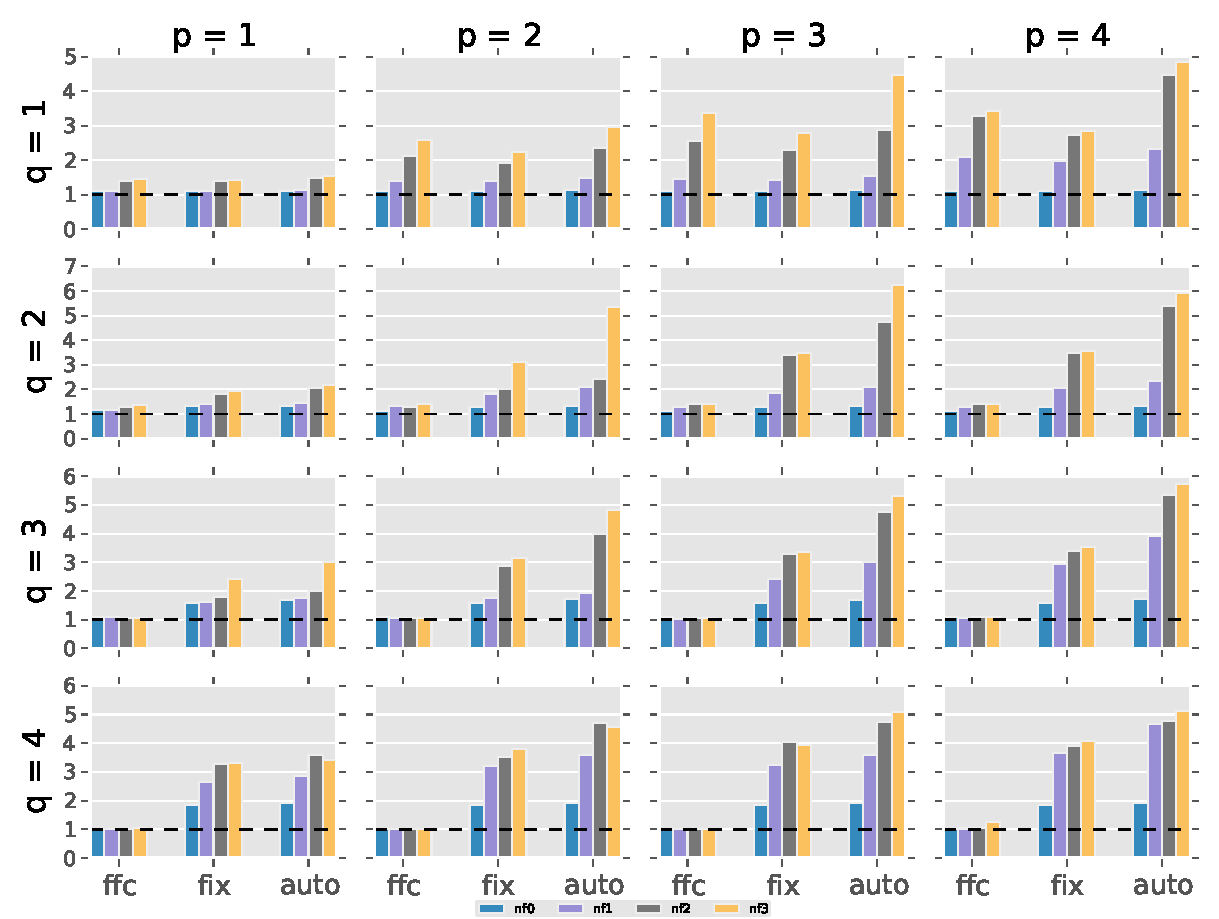
\includegraphics[scale=0.7]{coffee/perf-results/allforms/elasticity}}
\caption{Elasticity results.}\label{fig:coffee-allforms-elasticity}
\end{figure}
Figure~\ref{fig:coffee-allforms-elasticity} illustrates results for the Elasticity problem. This form uses a vector-valued space for the basis functions, so here transformations avoiding computation over zero-valued columns are of key importance. The \texttt{ffc} set of optimizations leads to notable improvements over the original code at $q=1$. The use of inderection arrays allows to phisically eliminate zero-valued columns at code generation time; as a consequence, different tabulated basis functions are merged into a single array. Therefore, despite the execution being purely scalar because of indirection arrays, the reduction in arithmetic intensity and register pressure imply improvement in performance. Nevertheless, \texttt{auto} remains in general the best choice, with gains over \texttt{ffc} that are wider as $p$ and $nf$ increase. 

For $q \geq 2$, in \texttt{ffc} the lack of SIMD vectorization counterbalances the decrease in the number of floating point operations, leading to speed ups over the original code that only occasionally exceed 1$\times$. On the other hand, the successful application of the zero-avoidance optimization while preserving code specialization plays a key role for \texttt{auto}, resulting in much higher performance code especially at $q=2$ and $q=3$. 

It is worth noting that speed ups of \texttt{auto} over \texttt{fix} decrease at $q=4$, particularly for low values of $p$. As we will discuss in Section~\ref{sec:coffee-pereval-autotune}, this is because at $q=4$ the vector-register tiling transformation (in combination with loop unroll-and-jam) leads to the highest performance. In principle, vector-register tiling can be used in combination to the zero-avoidance technique; however, due to mere technical limitations, this is currently not supported in COFFEE. Once solved, we expect much higher speed ups in the $q=4$ regime as well.

% TODO: mention aggressive expression rewriting somewhere

\subsection{Performance of Poisson}
\begin{figure}[t]
\centerline{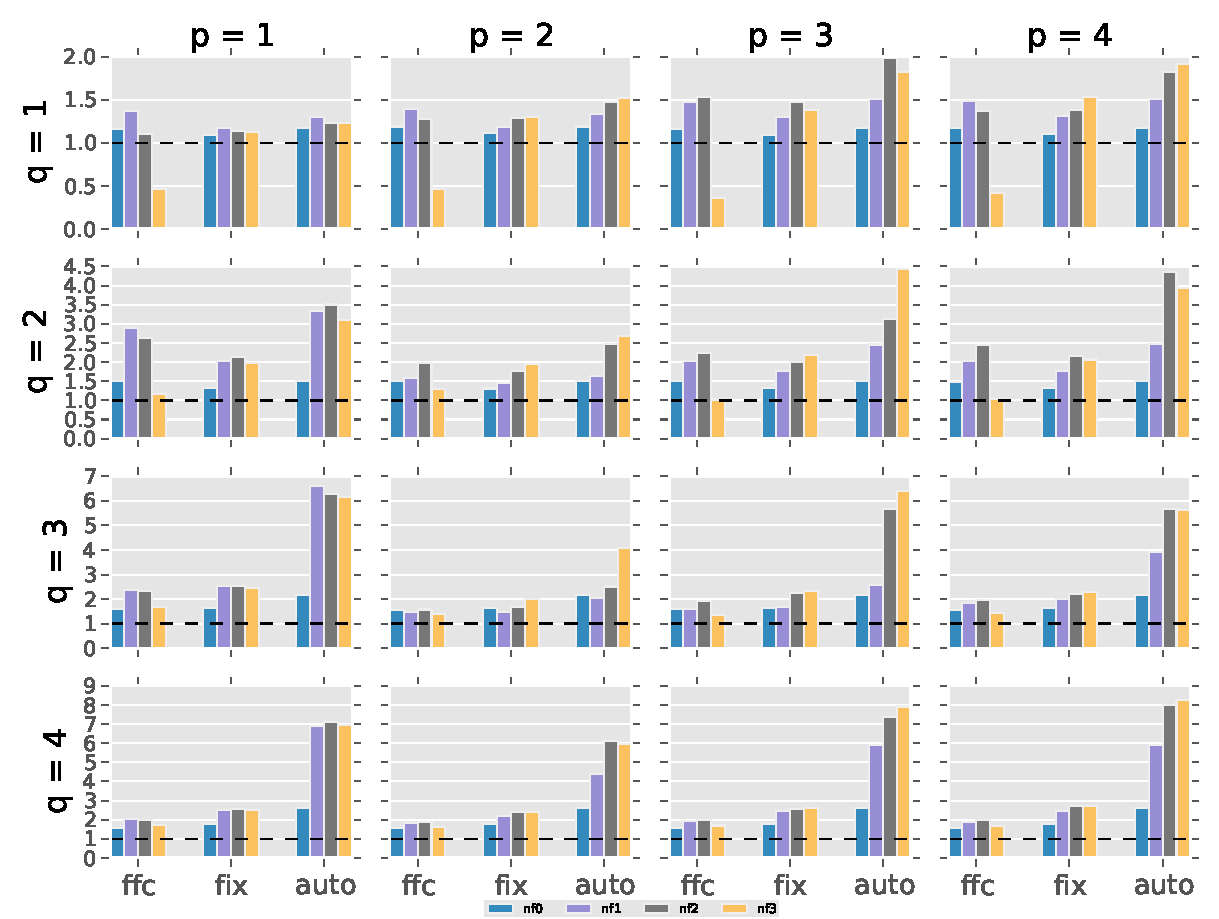
\includegraphics[scale=0.7]{coffee/perf-results/allforms/poisson}}
\caption{Poisson results.}\label{fig:coffee-allforms-poisson}
\end{figure}

In Figure~\ref{fig:coffee-allforms-poisson} we report speed ups of \texttt{ffc}, \texttt{fix}, and \texttt{auto} over the original code for the Poisson form. We note that, as a general trend, \texttt{ffc} exhibits drops in performance as $nf$ increases, notably when $nf=3$, for any values of $q$ and $p$. This is a consequence of the inherent complexity of the generated code. The way \texttt{ffc} performs loop-invariant code motion leads to the pre-computation of integration-dependent terms at the level of the integration loop, which are characterized by higher arithmetic intensity and redundant computation as $nf$ increases. Moreover, the absence of vectorization is another limiting factor.

The \texttt{auto} variant generally shows the best performance. Significant improvements over \texttt{fix} are also achieved, notably as $q$, $p$ and $nf$ increase. As clarified in the next section, this is always due to a more aggressive expression rewriting in combination with the zero-avoidance technique.


\subsection{Performance of Hyperelasticity}
\begin{figure}[t]
\centerline{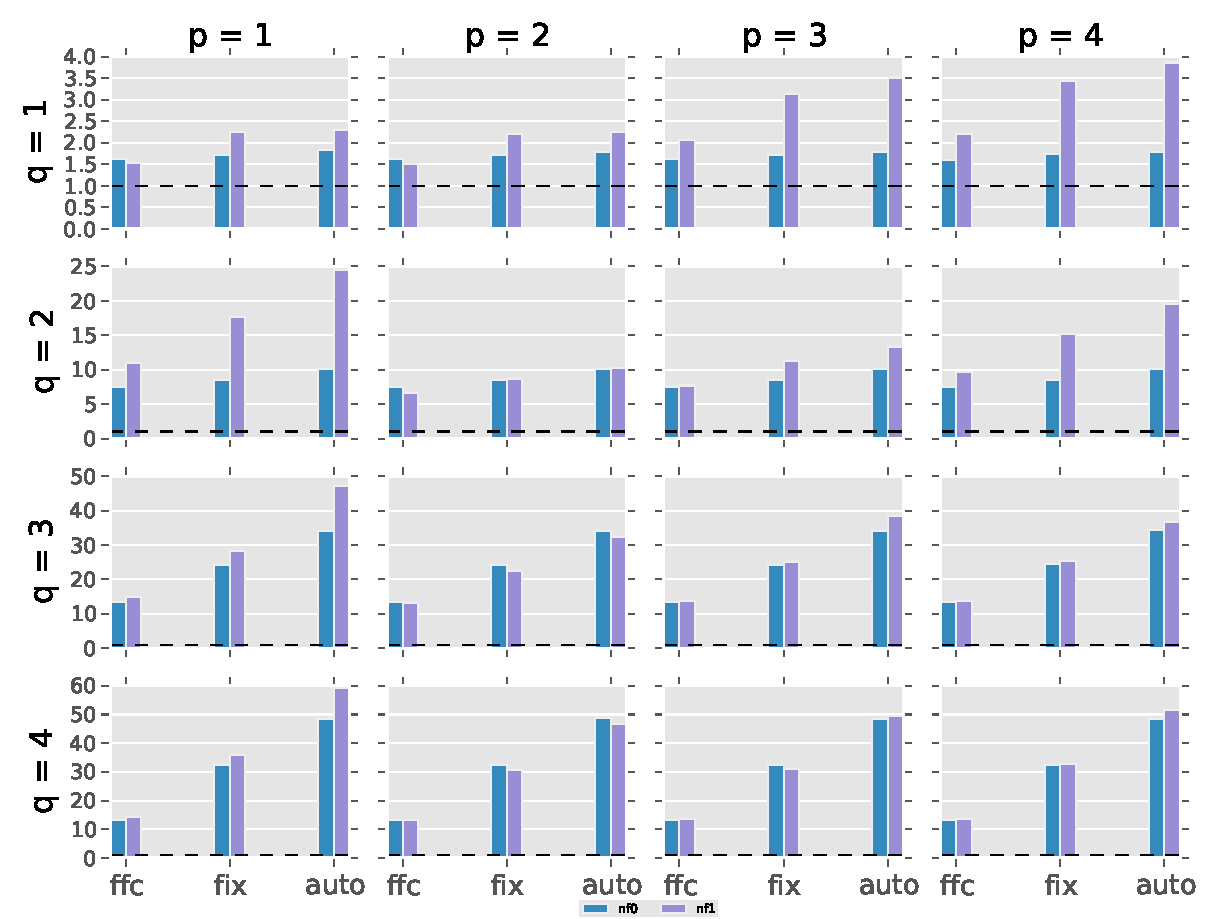
\includegraphics[scale=0.7]{coffee/perf-results/allforms/hyperelasticity}}
\caption{Hyperelasticity results.}\label{fig:coffee-allforms-hyperelasticity}
\end{figure}

Speed ups for the hyperelasticity form are shown in Figure~\ref{fig:coffee-allforms-hyperelasticity}. Experiments for $nf \geq 2$ could not be executed because of FEniCS-Form-Compiler's technical limitations. 

For \texttt{auto}, massive speed ups for $q \geq 2$ are to be ascribed to aggressive and successful expression writing. Hyperelasticity problems are really compute-intensive, with thousands of operations being performed, so reductions in redundant and useless computation are crucial. Complex forms like hyperelasticity would benefit from further ``specialized'' optimizations: for example, it is a known technical limitation of COFFEE that, in some circumstances, less temporaries could (should) be generated and that hoisted code could (should) be suitably distributed over different loops to minimize register pressure (e.g. COFFEE could apply loop fission for obtaining significantly better register usage). We expect to obtain considerably faster code once such optimizations will be incorporated. 

In the regime $q \geq 2$ and $nf=1$, peformance improvements are less pronounced moving from $p=1$ to $p=2$, although still significant; in particular, we notice a drop at $p=2$, followed by a raise up to $p=4$. It is worth observing that this effect is common to all sets of optimizations. The hypothesis is that this is due to the way coefficient functions are evaluated at quadrature points (identical in all configurations), which cannot be easily vectorized unless a change in storage layout and loops order is implemented in the code (abstract syntax tree) generator on top of COFFEE. 

\subsection{Details on the Autotuning Process}
\label{sec:coffee-pereval-autotune}

\subsubsection{Autotuning Overhead}
We first comment on the overhead of the autotuning process. In the context of Firedrake, the framework in which COFFEE is integrated, the autotuner is executed at run-time, once the local assembly kernels are provided by the FEniCS Form Compiler. Autotuning, therefore, introduces an overhead in the application execution time. Such overhead originates from four operations: 1) creation of the various code variants; 2) generation of a C file containing such variants (as simple function calls, plus the ``main'' function that invokes the variants, in sequence); 3) compilation of the autotuning file; 4) execution. Of these four points, we note that: the cost of 4) is relatively small, because each variant's execution time is bound by an empirically-found value (e.g. some milliseconds). The cost of all four points is constrained by our heuristics to prune the search space, as described in Section~\ref{sec:coffee-autotune}. Moreover, for a given form and a given discretization, the autotuner needs to be executed only once, since its output is saved and reused for later assemblies. This implies that if the assembly occurs in a time stepping loop, or the same form is executed on a different mesh, or known quantities of the input problem are changed, then the assembly cost is rapidly amortized. Premised that, the most important thing remains that when working with real unstructured meshes - which are likely to be composed of millions of elements, leading to long-lasting assembly phases - the autotuner overhead practically becomes completely negligible. In our experience, and in particular in the four examined problems, the autotuning process lasted less than a minute in the majority of cases. Most often, it took less than thirty seconds. Rarely it needed more than a minute, as for instance in the case of hyperelasticity; however, despite the inherent complexity of this form, we measured a peak of only 4 minutes for the extreme case $[q=4, p=4, nf=1]$, while 1.30 minutes were needed in the case $[q=1, p=1, nf=1]$. This analysis certifies that the autotuner overhead is definitely sustainable in real-world applications.

\subsubsection{Selected Optimizations}
We have repeatedly claimed that different forms (and different discretizations) require distinct sets of transformations to reach close-to-peak performance. To demonstrate this, we now report details about the output of the autotuning process. We show that for the four examined forms - more specifically, for the 224 problem instances $[form, q, p, nf]$ illustrated in the previous figures - a plethora of optimization strategies have been selected by the autotuner. We also complement and strengthen our claim by showing the autotuner's output for two additional forms whose performance results, for brevity, were not shown in Section~\ref{sec:coffee-allforms-perf}: a Mass and a Mixed Poisson problems. 

Table~\ref{table:autotuner-output} shows the number a given transformation has been selected by the autotuner. To not hinder readability, the output has been grouped by form, rather than showing the selected optimization strategy for each $[form, q, p, nf]$. Values in the \texttt{rewrite strategy} column can either be \texttt{base} or \texttt{aggressive}, as explained in Section~\ref{sec:coffee-autotune}: in the former case, only generalized loop-invariant code motion in applied; in the latter case, the rewrite rules are recursively applied, as extensive as possible. If the value is \texttt{aggressive} (\texttt{base}) it means that in the majority of cases the \texttt{aggressive} (\texttt{base}) strategy prevailed on the \texttt{base} (\texttt{aggressive}) one. Precomputation of integration-dependent terms was explained in Section~\ref{sec:coffee-precompute}. The \texttt{split} column refers to the expression splitting transformation (Section~\ref{sec:coffee-split}). The \texttt{unroll} column indicates the application of explicit unrolling. Other columns are of obvious meaning. Values in the various cells illustrate the number of problem instances (out of the total reported in column \texttt{number of variants}) in which an optimization was activated. Obviously, more transformations are typically used in combination in a same problem. 

\begin{table*}
\tiny
\centerline{\begin{tabulary}{1.0\textwidth}{c|c|ccc|ccccc}
\cline{3-10}
\multicolumn{2}{c}{} & \multicolumn{3}{c|}{\texttt{expression rewriting}} & \multicolumn{5}{c}{\texttt{code specialization}} \\
\cline{1-10}
problem & \specialcell{number of\\variants} & \specialcell{rewrite\\strategy} & \specialcell{zero-valued\\columns\\avoidance} & \specialcell{precompute\\integration terms} & \specialcell{padding\\alignment} & split & \specialcell{vector\\register\\tiling} & unroll & BLAS \\
\cline{1-10}
\texttt{helmholtz} & 64 & aggressive & 0 & 0 & all & 12 & 26 & 20 & 0 \\
\texttt{mass} & 64 & base & 0 & 0 & all & 0 & 0 & 31 & 2 \\
\texttt{elasticity} & 64 & aggressive & 39 & 0 & all & 0 & 11 & 0 & 2 \\
\texttt{poisson} & 64 & aggressive & 52 & 0 & all & all & 0 & 0 & 0 \\
\texttt{mixed poisson} & 192 & base & 0 & 0 & all & 32 & 68 & 36 & 0 \\
\texttt{hyperelasticity} & 32 & aggressive & all & all & all & 2 & 0 & 0 & 0 \\
\cline{1-10}
\end{tabulary}}
\caption{Summary of the optimizations selected by the autotuner in a number of forms}
\label{table:autotuner-output}
\end{table*}

\subsection{Full Application Study}
\label{sec:coffee-pereval-fullapp}

In this section, we investigate the performance gain for an entire finite element computation developed in Firedrake, a linear elasticity problem. The source code is available at~\cite{elasticity-code}. The equation is used to simulate deformation of an object caused by pre-established loading conditions.

The execution time of a steady finite element problem is dominated by two factors: assembly and solve. The evaluation of all local element matrices and vectors, and their insertion, respectively, in a ``global'' sparse matrix and a global vector, compose the ``assembly'' phase. The global matrix and vector form a linear system, usually solved by an iterative method; this is the ``solve'' phase. The percentage of time spent in assembly and solve varies from problem to problem. As reiterated in the available literature, for example in~\cite{quadrature1}, the computational cost of local assembly grows with the \textit{complexity} of the partial differential equation (e.g. because of larger loops and more articulated expressions), while the solve time increases with polynomial order and mesh discretization. The complexity of an equation depends on several factors, including the number of derivatives and coefficient functions (i.e. additional known functions that characterize the equation).

We study two versions of the static linear elasticity problem: 1) with one coefficient function, $f=1$, and 2) with two coefficient functions, $f=2$. More coefficient functions are also plausible; however, as we will see, the assembly process starts being particularly expensive already with $f=1$. For each of these two versions, we examine the cases of polynomial order $q=1$ and $q=2$. To run our experiments, we use a single core of the Sandy Bridge architecture described in Section~\ref{sec:perf-results}. The application runs on a tetrahedral mesh composed of 196608 elements.

\begin{figure}
	\centering
	\subfigure[]{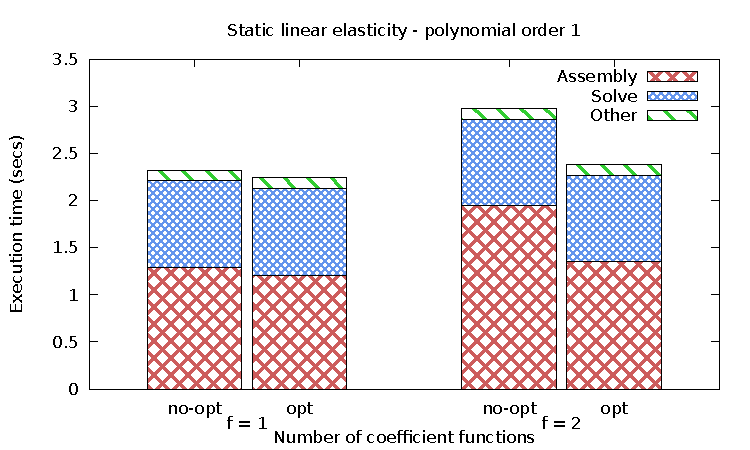
\includegraphics[scale=0.48]{coffee/perf-results/full-app/elasticity-p1.pdf}}
	\subfigure[]{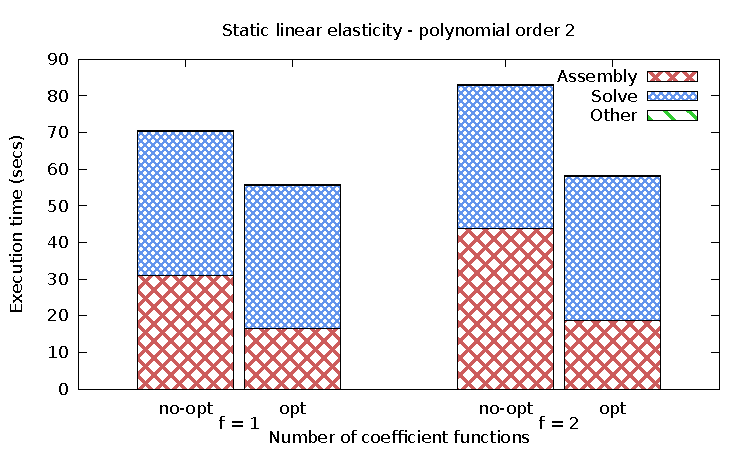
\includegraphics[scale=0.48]{coffee/perf-results/full-app/elasticity-p2.pdf}}
	\caption{Performance improvement over non-optimized code for the static linear elasticity equation on a single core of the Sandy Bridge architecture.}
	\label{fig:full-app-res}
\end{figure}

In Figure~\ref{fig:full-app-res}, we show the execution times for the four test cases, split over two figures (one for each polynomial order), without and with optimizations enabled. A stacked bar captures the time spent in the assembly phase (\texttt{assembly}), in solving the linear system (\texttt{solve}), and in the other various parts of the program (\texttt{other} - for example, setup of the problem and initialization of the coefficient functions). The \emph{non-opt} and \emph{opt} bars correspond, respectively, to the cases in which no optimizations and a combination of optimizations have been applied. The optimizations applied are generalized loop-invariant code motion, alignment and padding, and expression splitting. We recall that the cost of the insertion of the computed local element matrices (and vectors) in the global matrix (vector) is incorporated in \texttt{assembly}.

We first notice that, in the scenario ($f=1, p=1$), the assembly is dominated by matrix insertion: despite the application of several transformations, only a minimal performance gain is achieved. However, if either $q$ or $f$ is increased then the cost of \texttt{assembly} becomes larger with respect to \texttt{solve}, and the matrix insertion cost becomes negligible. In such cases, the transformations automatically applied by COFFEE dramatically decrease the cost of \texttt{assembly}. This results in
a significant overall speedup and a simulation which is now dominated by \texttt{solve} time. It is interesting to note that generalized loop-invariant code motion was particularly invasive in this case, with 23 temporaries generated and several redundancies discovered.

In these experiments, we observe a maximum performance improvement of 1.47$\times$ over the non-optimized local assembly code, obtained in the case ($f=2, p=2$). However, we reiterate the fact that full application speed ups increase proportionally with the amount of time spent in assembly and, therefore, with the complexity of the equation. By
increasing polynomial order and number of coefficient functions, or by simply studying a different, more complex equation, it is our experience that performance gains become increasingly more relevant. The choice of studying the static linear elasticity equation was to show that even relatively simple problems can be characterized by a large proportion of execution time spent in assembly. 

\section{Related Work}
\label{sec:coffee-related-work}
The finite element method is extensively used to approximate solutions of PDEs. Well-known frameworks and applications include nek5000~\cite{nek5000-web-page}, the FEniCS project~\cite{Fenics}, Fluidity~\cite{fluidity_manual_v4}, and of course Firedrake. Numerical integration based on quadrature, as in Firedrake, is usually employed to implement the local assembly phase. The recent introduction of domain specific languages (DSLs) to decouple the finite element specification from its underlying implementation facilitated, however, the development of novel approaches. Methods based on tensor contraction~\citep{FFC-Compiler} and symbolic manipulation~\citep{francis} have been implemented. Nevertheless, it has been demonstrated that quadrature-based integration remains the most efficient choice for a wide class of problems~\citep{quadrature-olegaard}, which motivates our work in COFFEE.

Optimization of quadrature-based local assembly for CPU architectures has been addressed in FEniCS~\cite{quadrature-olegaard}. The comparison between COFFEE and this work has been presented in Section~\ref{sec:coffee-allforms-perf}. In~\citep{Markall20101815}, and more recently in~\citep{petsc-integration-gpu}, the same problem has been studied for GPU architectures. In~\citep{assembly-opencl}, variants of the standard numerical integration algorithm have been specialized and evaluated for the PowerXCell processor, but an exhaustive study from the compiler viewpoint - like ours - is missing, and none of the optimizations presented in this chapter are mentioned. Among these efforts, to the best of our knowledge, COFFEE is the first work targeting low-level optimizations through a real compiler approach.

The code transformations presented are inspired by standard compilers optimizations and exploit domain properties. Our loop-invariant code motion technique individuates invariant sub-expressions and redundant computation by analyzing all loops in an iteration space, which is a generalization of the algorithms often implemented by general-purpose compilers. Expression splitting is an abstract variant of loop fission based on properties of arithmetic operators. The outer-product vectorization is an implementation of tiling at the level of vector registers; tiling, or ``loop blocking'', is commonly used to improve data locality (especially for caches). Padding has been used to achieve data alignment and to improve the effectiveness of vectorization. A standard reference for the compilation techniques re-adapted in this work is~\citep{dragonbook}.

Our compiler-based optimization approach is made possible by the top-level DSL, which enables automated code generation. DSLs have been proven successful in auto-generating optimized code for other domains: Spiral~\citep{Pueschel:05} for digital signal processing numerical algorithms, ~\citep{Spampinato:14} for dense linear algebra, or Pochoir~\cite{pochoir} and SDSL~\cite{stencil-compiler} for image processing and finite difference stencils. Similarly, PyOP2 is used by Firedrake to express iteration over unstructured meshes in scientific codes. COFFEE improves automated code generation in Firedrake.

Many code generators, like those based on the Polyhedral model~\cite{pluto} and those driven by domain-knowledge~\cite{modeldriven}, make use of cost models. The alternative of using auto-tuning to select the best implementation for a given problem on a certain platform has been adopted by nek5000~\cite{nek5000} for small matrix-matrix multiplies, the ATLAS library~\cite{ATLAS}, and FFTW~\cite{FFTW} for fast fourier transforms. In both cases, pruning the implementation space is fundamental to mitigate complexity and overhead. Likewise, COFFEE uses heuristics and a model-driven auto-tuning system (Section~\ref{sec:coffee-autotune}) to steer the optimization process.


\section{Generality of the Approach and Applicability to Other Domains}
\label{sec:generality}
We have demonstrated that our cross-loop optimizations for arithmetic intensity are effective in the context of automated code generation for finite element local assembly. In this section, we discuss their applicability in other computational domains and, in general, their integrability within a general-purpose compiler.

COFFEE was developed as a separate, self-contained software module, with clear input/output interfaces, rather then incorporating it within PyOP2. This choice was motivated by two critical aspects that characterize the generality of our research:

\paragraph{Separation of concerns} We believe that in domain-specific frameworks there must be a clear, logical separation of roles reflecting the various levels of abstraction, where domain specialists are completely separated from performance optimization. In Firedrake, for instance, COFFEE decouples the mathematical specification of a finite element method, captured by the Unified Form Language and the FEniCS Form Compiler, from code optimization. This is of fundamental importance to maximize productivity by allowing scientists to focus only on their area of expertise. Practically speaking, from the perspective of the domain-specific language and compiler designers, our optimization strategy represents an incentive to produce extremely simple representations of the code (e.g. fully-inlined mathematical expressions in the form of an abstract syntax tree, in the case of Firedrake) so as to make the architecture-aware code optimizer completely responsible for choosing and applying the most suitable set of transformations.

\paragraph{Generalizability to other domains} There are neither conceptual nor technical reasons which prevent our compiler from being used in applications other than Firedrake. For example, integration with the popular FEniCS framework, the pioneer of automated code generation for finite element local assembly, would be relatively easy to achieve. It is more challenging to assess the generality of the optimization strategy: the extent to which COFFEE and its transformations are transferable to other computational domains, perhaps other DSLs, and to what extent this would be helpful for improving full application performance. To answer these questions, we first need to go back to the origins of our compiler. The starting point of our work was the mathematical formulation of a local assembly operation, expressible as follows

\begin{equation}
\label{eq:assembly-model}
\scriptsize
\forall_{i, j} ~~~ A_{ij}^K = \sum_{q=1}^{n_1} \sum_{k=1}^{n_2} \alpha_{k, q}(a', b', c', ...) \beta_{q, i, j}(a, b, c, d, ...) \gamma_{q}(w_K, z_K)
\end{equation}

The expression represents the numerical evaluation of an integral at $n_1$ points in the mesh element $K$ computing the local element matrix $A$. Functions $\alpha$, $\beta$ and $\gamma$ are problem-specific and can be intricately complex, involving for example the evaluation of derivatives. We can however abstract from the inherent structure of $\alpha$, $\beta$ and $\gamma$ to highlight a number of aspects

\begin{itemize}
\item \textbf{Optimizing mathematical expressions.} Expression manipulation (e.g. simplification, decomposition into sub-expressions) opens multiple semantically equivalent code generation opportunities, characterized by different trade-offs in parallelism, redundant computation, and data locality. The basic idea is to exploit properties of arithmetic operators, such as associativity and commutativity, to re-schedule the computation suitably for the underlying architecture. Loop-invariant code motion and expression splitting follow this principle, so they can be re-adapted or extended to any domains involving numerical evaluation of complex mathematical expressions (e.g. electronic structure calculations in physics and quantum chemistry relying on tensor contractions~\cite{TCE}). In this context, we highlight three notable points.
\begin{enumerate}
\item In Equation~\eqref{eq:assembly-model}, the summations correspond to reduction loops, whereas loops over indices $i$ and $j$ are fully parallel. Throughout the paper we assumed that a kernel will be executed by a single thread, which is likely to be the best strategy for standard multi-core CPUs. On the other hand, we note that for certain architectures (for example GPUs) this could be prohibitive due to memory requirements. Intra-kernel parallelization is one possible solution: a domain-specific compiler such as COFFEE could map mathematical quantifiers and operators to different parallelization schemes and generate distinct variants of multi-threaded kernel code. Based on our experience, we believe this is the right approach to achieve performance portability.
\item The various sub-expressions in $\beta$ only depend on (i.e. iterate along) a subset of the enclosing loops. In addition, some of these sub-expressions might reduce to the same values as iterating along certain iteration spaces. This code structure motivated the generalized loop-invariant code motion technique. The intuition is that whenever sub-expressions invariant with respect to different sets of affine loops can be identified, the question of whether, where and how to hoist them, while minimizing redundant computation, arises. Pre-computation of invariant terms also increases memory requirements due to the need for temporary arrays, so it is possible that for certain architectures the transformation could actually cause slowdowns (e.g. whenever the available per-core memory is small).
\item Associative arithmetic operators are the prerequisite for expression splitting. In essence, this transformation concerns resource-aware execution. In the context of COFFEE, expression splitting has been successfully applied to improve register pressure. However, the underlying idea of re-scheduling (re-associating) operations to optimize for some generic parameters is far more general. It could be used, for example, as a starting point to perform kernel fission; that is, splitting a kernel into multiple parts, each part characterized by less stringent memory requirements (a variant of this idea for non-affine loops in unstructured mesh applications has been adopted in~\citep{carlolcpca}). In Equation~\eqref{eq:assembly-model}, for instance, not only can any of the functions $\alpha$, $\beta$ and $\gamma$ be split (assuming they include associative operators), but $\alpha$ could be completely extracted and evaluated in a separate kernel. This would reduce the working set size of each of the kernel functions, an option which is particularly attractive for many-core architectures in which the available per-core memory is much smaller than that in traditional CPUs.
\end{enumerate}
\item \textbf{Code generation and applicability of the transformations.} All array sizes and loop bounds, for example $n1$ and $n2$ in Equation~\ref{eq:assembly-model}, are known at code generation time. This means that ``good'' code can be generated. For example, loop bounds can be made explicit, arrays can be statically initialized, and pointer aliasing is easily avoidable. Further, all of these factors contribute to the applicability and the effectiveness of some of our code transformations. For instance, knowing loop bounds allows both generation of correct code when applying vector-register tiling and discovery of redundant computation  opportunities. Padding and data alignment are special cases, since they could be performed at run-time if some values were not known at code generation time. Theoretically, they could also be automated by a general-purpose compiler through profile-guided optimization, provided that some sort of data-flow analysis is performed to ensure that the extra loop iterations over the padded region do not affect the numerical results. 
\item \textbf{Multi-loop vectorization.} Compiler auto-vectorization has become increasingly effective in a variety of codes. However, to the best of our knowledge, multi-loop vectorization involving the loading and storing of data along a subset of the loops characterizing the iteration space (rather than just along the innermost loop), is not supported by available general-purpose and polyhedral compilers. The outer-product vectorization technique presented in this paper shows that two-loop vectorization can outperform standard auto-vectorization. In addition, we expect the performance gain to scale with the number of vectorized loops and the vector length (as demonstrated in  the Xeon Phi experiments). Although the automation of multi-loop vectorization in a general-purpose compiler is far from straightforward, especially if stencils are present, we believe that this could be more easily achieved in specific domains. The intuition is to map the memory access pattern onto vector registers, and then to exploit in-register shuffling to minimize the traffic between memory and processor. By demonstrating the effectiveness of multi-loop vectorization in a real scenario, our research represents an incentive for studying this technique in a broader and systematic way.
\end{itemize}

\section{Conclusion}
\label{sec:coffee-conclusion}
In this chapter, we have presented the study and systematic performance evaluation of a class of composable cross-loop optimizations for improving arithmetic intensity in finite element local assembly kernels, and their integration in a novel compiler, COFFEE. In the context of automated code generation for finite element local assembly, COFFEE is the first compiler capable of introducing low-level optimizations to maximize instruction-level parallelism, register locality and SIMD vectorization. Assembly kernels have particular characteristics. Their iteration space is usually very small, with the size depending on aspects like the degree of accuracy one wants to reach (polynomial order of the method) and the mesh discretization employed. The data space, in terms of number of arrays and scalars required to evaluate the element matrix, grows proportionally with the complexity of the finite element problem. COFFEE has been developed taking into account all of these degrees of freedom, based on the idea that reducing the problem of local assembly optimization to a fixed sequence of transformations is far too superficial if close-to-peak performance needs to be reached. The various optimizations overcome limitations of current vendor and research compilers. The exploitation of domain knowledge allows some of them to be particularly effective, as demonstrated by our experiments on a state-of-the-art Intel platform. COFFEE supports all of the problems expressible in Firedrake, and is integrated with this framework, which demonstrate the maturity of the research performed. The generality and the applicability of the proposed code transformations to other domains has also been discussed.